\documentclass{article}

% if you need to pass options to natbib, use, e.g.:
\PassOptionsToPackage{numbers, compress}{natbib}
% before loading neurips_2026

% The authors should use one of these tracks.
% Before accepting by the NeurIPS conference, select one of the options below.
% 0. "default" for submission
\usepackage{neurips_2026}

% the "default" option is equal to the "main" option, which is used for the Main Track with double-blind reviewing.
% 1. "main" option is used for the Main Track
%  \usepackage[main]{neurips_2026}
% 2. "position" option is used for the Position Paper Track
%  \usepackage[position]{neurips_2026}
% 3. "eandd" option is used for the Evaluations & Datasets Track
 % \usepackage[eandd]{neurips_2026}
 % if you need to opt-in for a single-blind submission in the E&D track:
 %\usepackage[eandd, nonanonymous]{neurips_2026}
% 4. "creativeai" option is used for the Creative AI Track
%  \usepackage[creativeai]{neurips_2026}
% 5. "sglblindworkshop" option is used for the Workshop with single-blind reviewing
 % \usepackage[sglblindworkshop]{neurips_2026}
% 6. "dblblindworkshop" option is used for the Workshop with double-blind reviewing
%  \usepackage[dblblindworkshop]{neurips_2026}

% After being accepted, the authors should add "final" behind the track to compile a camera-ready version.
% 1. Main Track
 % \usepackage[main, final]{neurips_2026}
% 2. Position Paper Track
%  \usepackage[position, final]{neurips_2026}
% 3. Evaluations & Datasets Track
 % \usepackage[eandd, final]{neurips_2026}
% 4. Creative AI Track
%  \usepackage[creativeai, final]{neurips_2026}
% 5. Workshop with single-blind reviewing
%  \usepackage[sglblindworkshop, final]{neurips_2026}
% 6. Workshop with double-blind reviewing
%  \usepackage[dblblindworkshop, final]{neurips_2026}
% Note. For the workshop paper template, both \title{} and \workshoptitle{} are required, with the former indicating the paper title shown in the title and the latter indicating the workshop title displayed in the footnote.
% For workshops (5., 6.), the authors should add the name of the workshop, "\workshoptitle" command is used to set the workshop title.
% \workshoptitle{WORKSHOP TITLE}

% "preprint" option is used for arXiv or other preprint submissions
 % \usepackage[preprint]{neurips_2026}

% to avoid loading the natbib package, add option nonatbib:
%    \usepackage[nonatbib]{neurips_2026}

\usepackage[utf8]{inputenc} % allow utf-8 input
\usepackage[T1]{fontenc}    % use 8-bit T1 fonts
\usepackage{hyperref}       % hyperlinks
\usepackage{url}            % simple URL typesetting
\usepackage{booktabs}       % professional-quality tables
\usepackage{amsfonts}       % blackboard math symbols
\usepackage{nicefrac}       % compact symbols for 1/2, etc.
\usepackage{microtype}      % microtypography
\usepackage{xcolor}         % colors
\usepackage{graphicx}
\usepackage{amsmath}
\usepackage{natbib}
\usepackage{subcaption}



% Note. For the workshop paper template, both \title{} and \workshoptitle{} are required, with the former indicating the paper title shown in the title and the latter indicating the workshop title displayed in the footnote.
%\title{TurboSens: An Interactive Turbofan Benchmark for World-Model Evaluation and Physical Understanding} % changé avec le titre ci-dessous pour simplifier:
\title{TurboSens: An Interactive Turbofan Benchmark for Probing World Models %Representations
against Ground Truth}
% \title{TurboSens: A Paired State Turbofan Benchmark for World Model Evaluation}



% The \author macro works with any number of authors. There are two commands
% used to separate the names and addresses of multiple authors: \And and \AND.
%
% Using \And between authors leaves it to LaTeX to determine where to break the
% lines. Using \AND forces a line break at that point. So, if LaTeX puts 3 of 4
% authors names on the first line, and the last on the second line, try using
% \AND instead of \And before the third author name.


\author{%
  Lucas Thil\thanks{Use footnote for providing further information about author (webpage, alternative address)---\emph{not} for acknowledging funding agencies.} \\
  LIX, École Polytechnique \\
  Palaiseau, France \\
  \texttt{lix@polytechnique.fr} \\
  \And
  IRT SystemX \\
  Palaiseau, France \\
  \texttt{lucas.thil@irt-systemx.fr} \\
  \AND
  Jesse Read \\
  LIX, École Polytechnique \\
  Palaiseau, France \\
  \texttt{jread@lix.polytechnique.fr} \\
  \AND
  Rim Kaddah \\
  IRT SystemX \\
  Palaiseau, France \\
  \texttt{rim.kaddah@irt-systemx.fr} \\
  \AND
  Guillaume Doquet \\
  Safran Tech \\
  Chateaufort, France \\
  \texttt{guillaume.doquet@safrangroup.com} \\
}

\begin{document}


\maketitle

% Suppress main body sections from the appendix TOC.
% Re-enabled right after \appendix below.
\addtocontents{toc}{\protect\setcounter{tocdepth}{-3}}

\begin{abstract}
Self supervised world models promise that representations learned from observations alone can recover the underlying generative state of a complex physical system. Verifying that they do is difficult when that state is unobserved: existing physics and prognostics benchmarks substitute a low dimensional readout (a plausibility verdict, a remaining useful life) that cannot certify what the representation actually preserved. We introduce TurboSens, an interactive turbofan simulator and dataset that supplies the missing ground truth. At every flight cycle, the simulator emits a sensor stream paired with the full ten dimensional health state of the engine, hidden behind sensor noise, fouling, and operating context confounds. This pairing enables a direct evaluation protocol that we call \emph{inverse probing}: a world model is pretrained on the sensor stream alone, the encoder is frozen, and a small supervised head, the \emph{probe}, is trained on top of the frozen embeddings to map them to the ground truth health state. The accuracy of this probe under in distribution and out of distribution (OOD) shifts measures how much of the underlying state the representation actually preserved. We release two progressively challenging scenarios (TurboSens1 and TurboSens2) along with a deterministic counterfactual replayer and reproducibility tooling. As an illustration, multi seed sweeps over two world model families, joint embedding predictive architectures (JEPA) and recurrent latent dynamics (autoregressive LSTM), show that lengthening the pretraining context (predictor history, encoder window, predictor stride) monotonically improves OOD probe quality across architectures, while a supervised oracle on the same encoder backbone closes the OOD gap entirely, situating the residual gap at the self supervised pretext rather than at the encoder backbone or the data.


% Alternative abstract
% \begin{abstract}
% Evaluating whether a world model recovers the underlying generative state of a physical system from observations alone is hard when that state is unobserved. Existing physics and prognostics benchmarks substitute a low dimensional readout (a plausibility verdict, a remaining useful life) that cannot certify what the representation preserved. We introduce TurboSens, an interactive turbofan simulator and dataset whose distinctive property is paired access to a sensor stream and the full ten dimensional engine health state at every flight cycle, structurally underdetermined by seven sensor channels and obscured by fouling, weather, and operating context confounds. The pairing supports an inverse probing protocol: a frozen self supervised encoder is probed against the ground truth through state estimation, distribution shift generalization, and counterfactual forecasting. Two progressively challenging scenarios are released alongside a deterministic replayer and multi seed reproducibility tooling. A demonstration sweep across two world model families shows that more temporal context during pretraining monotonically improves OOD probe quality and that a supervised oracle on the same backbone closes the OOD gap entirely, situating the residual gap at the self supervised pretext rather than the encoder backbone or the data.
% \end{abstract}


%World models learn representations of physical systems from observations, but evaluating whether they recover the underlying causal state is difficult when that state is unobserved. We introduce TurboSens, an interactive turbofan degradation simulator designed as an evaluation instrument for world model representations. It provides paired access to sensor streams and the full ground truth health state at every timestep: a ten dimensional latent underdetermined by seven sensors. This enables a direct protocol: train a self-supervised world model on observations alone, then evaluate its representations on state recovery, forecasting, and out of distribution generalization with action conditioning. We release two progressively challenging scenarios (TurboSens1 and TurboSens2) with configurable degradation, maintenance, a two channel hidden state, and a phantom observation map where sensed and true states diverge, to enable the community to build upon it.
%The turbofan domain offers complex, industry relevant dynamics: heterogeneous wear, sparse stochastic events, weather, and region specific conditions. Unlike pixel or language benchmarks, TurboSens provides ground truth, allowing us to ask what representations preserve under distribution shift, where failures originate (encoder vs predictor), and how temporal horizons affect robustness. As a demonstration, increasing the predictor horizon monotonically improves out of distribution generalization. The benchmark is released with reproducibility tooling, a counterfactual replayer, and documented assumptions, revealing a critical insight for world model design: out-of-distribution generalization requires temporally structured bottlenecks that preserve long horizon dependencies, not merely longer training contexts. Without ground truth access to the latent state, this dissociation between context length and bottleneck structure remains invisible.

\end{abstract}


\section{Introduction}
\label{sec:introduction}

% --- P1: the world-model evaluation question ---
World models~\cite{Balestriero_LeCun_2025, Assran_Bardes_Fan_Garrido_Howes_Mojtaba_Komeili_Muckley_Rizvi_Roberts_et_al_2025, okada2021dreaming, okada2022dreamingv2, Maes_Lidec_Scieur_LeCun_Balestriero_2026} are increasingly proposed as general purpose representations for complex dynamical systems, trained in a self-supervised manner to predict future state and spanning joint embedding, recurrent latent dynamics, and autoregressive architectures. A central open question is whether such representations recover the \emph{underlying generative} state of the system or merely fit statistical regularities of the observation stream. Answering this requires paired access to sensor observations \emph{and} the true latent state, which existing physics and prognostics benchmarks~\cite{bear1physion, riochet2018intphys, Bordes_Garrido_Kao_Williams_Rabbat_Dupoux_2025, Saxena_Goebel_Simon_Eklund_2008} replace by a low dimensional readout (a plausibility verdict, a scalar remaining useful life) that cannot certify whether a representation recovered the underlying generative structure.

% --- P2: what we provide (core instrument framing) ---
We introduce \textbf{TurboSens}, an interactive turbofan simulator and accompanying dataset designed as an \emph{instrument} for evaluating world‑model representations. TurboSens is generated using OpenDeckSMR~\cite{psaropoulos_2025_17804895}, a component‑level thermodynamic aircraft engine simulator that exposes, at every timestep, both a sensor stream and the full ten‑dimensional ground‑truth health state $\mathbf{s}_t$. This paired access enables an \emph{inverse evaluation protocol}: train a world model self‑supervised on sensor sequences alone, freeze the encoder, then probe the latent space against the true $\mathbf{s}_t$ through regression, forecasting, and out‑of‑distribution tasks. Because the true state is available but never used as a training signal, TurboSens asks whether a learned representation recovers the underlying generative state of engine health from observations alone, going beyond scalar RUL regression and binary violation‑of‑expectation discrimination.

\begin{figure}[t]
    \centering
    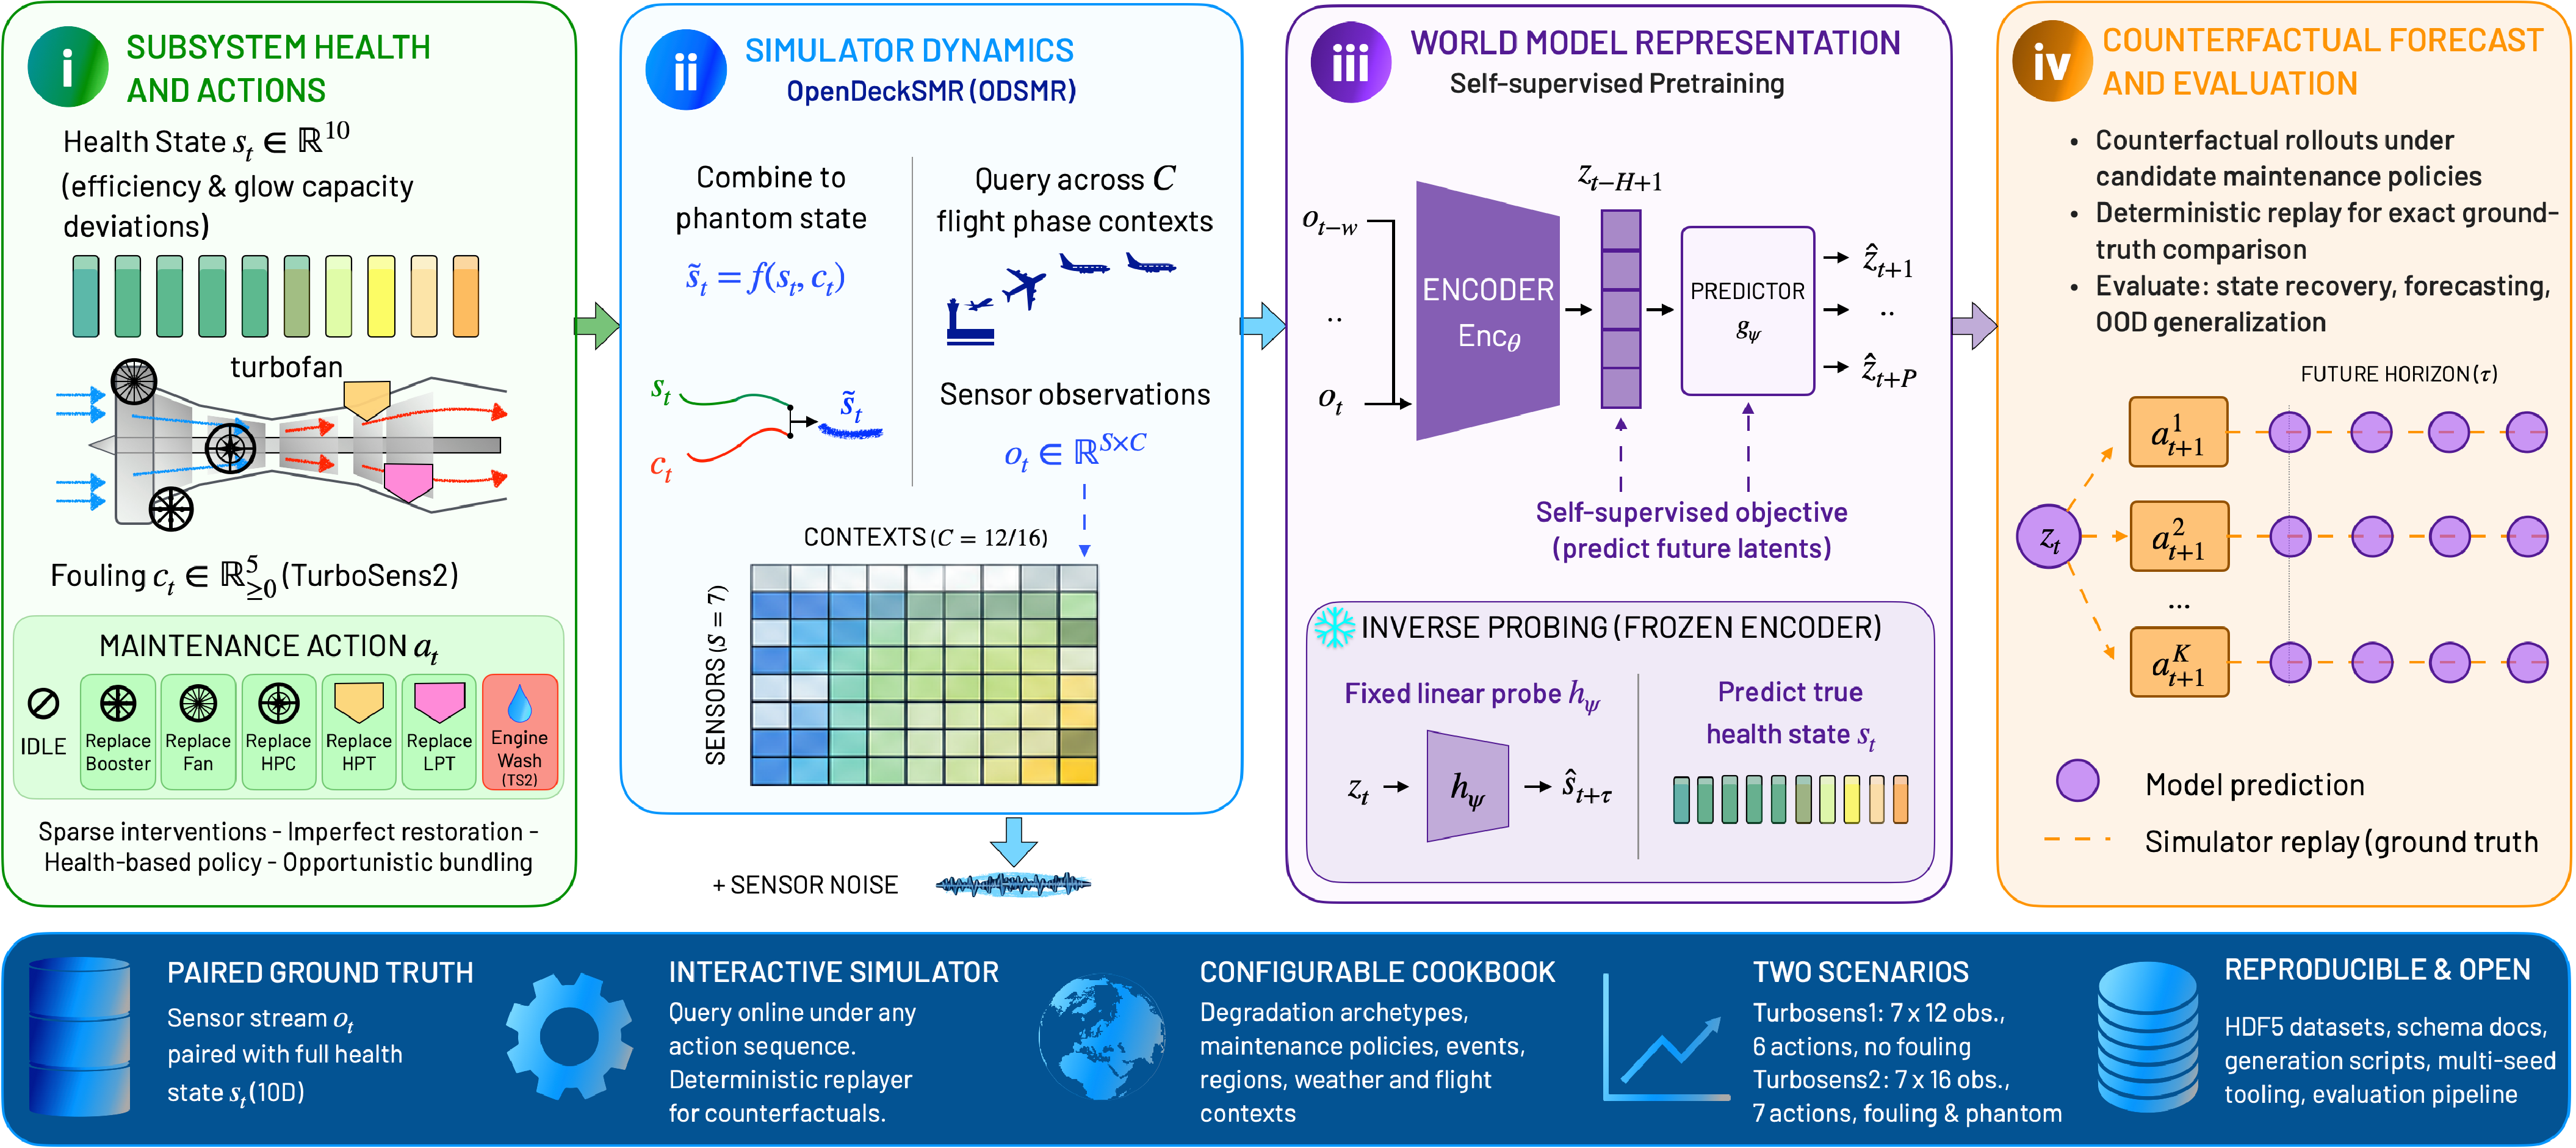
\includegraphics[width=1\linewidth]{figures/Turbosens1v4.pdf}

    \caption{\textbf{The TurboSens evaluation framework.} \textbf{(i)}~A turbofan engine is decomposed into subsystems whose health $\mathbf{s}_t \in \mathbb{R}^{10}$ degrades over time and is partially restored by discrete maintenance actions $a_t$; a fouling channel $\mathbf{c}_t$ accumulates between washes (TurboSens2 only). \textbf{(ii)}~The two channels combine into a phantom state $\tilde{\mathbf{s}}_t = f(\mathbf{s}_t, \mathbf{c}_t)$ that OpenDeckSMR (ODSMR) maps to sensor observations $\mathbf{o}_t \in \mathbb{R}^{S \times C}$ across $C$ flight phase contexts. \textbf{(iii)}~A world model is pretrained self supervised (encoder $\mathrm{Enc}_\theta$, predictor $g_\psi$); at evaluation the encoder is frozen and a small supervised head trained on its embeddings, which we call a \emph{probe} ($h_\psi$), decodes them against the ground truth $\mathbf{s}_t$. \textbf{(iv)}~Counterfactual forecasting forks an episode under alternative actions $\{a^k_{t+1}\}$ and compares the model's rollout against a deterministic simulator replay over a future horizon $\tau$.}

    %\caption{\textbf{The Turbosens evaluation framework. A) The latent state} $\omega_t$ packs sub-system health state $s_t$ (green per subsystems), fouling $c_t$ (red diamonds) adds a degradation deposit on the sub-systems states. Maintenance action $a_t$ (pink) restore the health of some systems, or reduces fouling. Weather and phase contexts ($w_t,\phi_t$) (yellow) condition the environment. \textbf{B) Simulator dynamics and world model:} OpenDeckSMR emits a sensor observation $o_t=g(\omega_t)$ at every timestep, and a self supervised world model learns to encode $o_t$ into a latent $z_t$ that is advanced by the predictor under the action history. \textbf{C) Possible futures forecasting and inverse probing:} branching from $z_t$ under alternative actions $a_{t+1}$ produces predicted future latents that we compare against the simulator's deterministic replay; a fixed head $h_\psi$ maps $z_t$ to the simulator's ground truth state $s_t$ over multiple horizons.}
    \label{fig:problem_formulation}
\end{figure}



% --- P3: interactive instrument + state structure (merged P3+P4) ---
TurboSens is \emph{interactive} rather than a static dump of trajectories: the simulator can be queried online under arbitrary action sequences for counterfactual rollouts and on-demand generation of out-of-distribution regimes, with degradation archetypes, maintenance policies, event rates, and flight phase contexts exposed as independent knobs. The simulator is driven by a well-maintained fleet abstraction (life-limiting part ceilings, health correlated scheduling, opportunistic bundling, imperfect restoration), so trajectories unfold as a \emph{sawtooth of partial resets} punctuated by rare stochastic events; sensor observations are recorded across multiple flight phase contexts per timestep and the seven-channel observation is structurally underdetermined relative to the ten state dimensions. Even if every modeling element draws grounds in industrial operating practice, it is not representative of a real serviced engine. We make these choices documented and configurable, so users can audit our assumptions independently of the protocol.

% --- P5: Contributions ---
\paragraph{Contributions.}
\begin{enumerate}
    \item An \textbf{interactive turbofan simulator} built on OpenDeckSMR, exposing paired ground‑truth state and sensor observations with discrete maintenance actions, on‑demand trajectory generation, and a configurable cookbook of degradation archetypes, maintenance policies, events, and flight contexts.

    \item An \textbf{inverse evaluation protocol (`probing')} that trains world models self‑supervised on sensor sequences, then directly probes their representations against the full ten‑dimensional health state through regression, degradation‑velocity estimation, multi‑step latent forecasting, and out of distribution (OOD) detection.

    \item \textbf{Reference scenarios and splits}: released HDF5 datasets (TurboSens1, TurboSens2) with documented schemas, providing a concrete starting point for the protocol while leaving the pipeline open for further scenario composition.
\end{enumerate}






\section{Related Work}
\label{sec:related_work}

\paragraph{Why turbofan engines.}
Turbofan operation is a high stakes domain in which the degradation mechanisms driving wear are only partially observable through sensors, motivating a substrate where representation quality can be measured against an exposed ground truth state. We pick this substrate for world model evaluation for three reasons. First, the observations are scalar sensor channels rather than pixels, which removes the visual decoding bottleneck that dominates evaluation on video benchmarks and isolates the question of whether the encoder captures the underlying generative state. Second, the system carries a physically meaningful latent state (component level efficiency and flow capacity deviations) \cite{lacaille2014robust, karchmer1977identification} that the simulator emits at every timestep, so a probe against the ground truth state is well-posed and component-identifiable. Third, a single engine simultaneously exercises many phenomena \cite{riegler2007geared, dunn1987performance, thoma2020quantifying, aygun2024thermodynamics} that world models must handle in concert: noise, multi-context observations, action interventions through maintenance, region and phase-dependent dynamics, and rare stochastic events. The turbofan substrate also bridges world model evaluation with the predictive maintenance \cite{zonta2020predictive, lee2014prognostics, tsui2015prognostics, jaw2005recent} and digital twin literature \cite{mihai2022digital, Belfadel_Creff_Ben_Hamida_2025}, but the goal of this paper is squarely the former; the dataset is positioned as an instrument for evaluating world model representations, not as a prognostics benchmark.


\paragraph{World models and physical understanding.}
A growing family of world models, spanning joint‑embedding predictive architectures~\cite{Balestriero_LeCun_2025, Assran_Bardes_Fan_Garrido_Howes_Mojtaba_Komeili_Muckley_Rizvi_Roberts_et_al_2025, Maes_Lidec_Scieur_LeCun_Balestriero_2026}, recurrent latent‑dynamics models~\cite{okada2021dreaming, okada2022dreamingv2}, and autoregressive sequence models~\cite{wang2020data, krishnan2022self, deng2024enhancing, calabrese2021predictive}, train encoders and predictors on high‑dimensional observation streams (pixels, sensors) to recover latent dynamics without supervision. A parallel body of work asks whether such representations encode \emph{physical} structure: Physion~\cite{bear1physion} scores rigid‑body outcome prediction, CLEVRER~\cite{yiclevrer} probes causal reasoning over collision videos, and IntPhys/IntPhys2~\cite{riochet2018intphys, Bordes_Garrido_Kao_Williams_Rabbat_Dupoux_2025} adopt a violation‑of‑expectation paradigm. Two structural limitations recur across the field. First, these evaluations reduce physical understanding to binary discrimination, effectively an out‑of‑distribution detection task that flags anomalies rather than recovering the underlying state. Second, ground‑truth access to the latent state is typically unavailable, so evaluation collapses onto downstream task return or reconstruction quality and cannot certify whether the representation captures physical structure or merely statistical regularities of the observation stream.

\paragraph{Interactive simulators and agentic environments.}
Gym‑style interactive environments are the standard testbed for reinforcement learning and model predictive control~\cite{towers2024gymnasium, todorov2012mujoco}, but industrial degradation settings have received comparatively little attention in this form. \citet{Maulana_Starr_Ompusunggu_2023} argue for maintenance policies that reason over longer action horizons, a setting that requires an online simulator rather than a static dataset. No existing turbofan benchmark exposes this interface: an agent cannot apply a maintenance action and observe the consequence.

\paragraph{Turbofan degradation datasets.}
Turbofan prognostics research has long been dominated by C‑MAPSS~\cite{Saxena_Goebel_Simon_Eklund_2008} and N‑CMAPSS~\cite{Arias_Chao_Kulkarni_Goebel_Fink_2021}, which pair sensor streams with a scalar remaining‑useful‑life label as the sole evaluation target~\cite{Ramasso_Saxena}. These datasets established the field but expose neither the full latent health state nor an interactive interface.

% Piloto_Weinstein_Battaglia_Botvinick_2022


\section{Problem Formulation: Turbofan Degradation and Simulator}
\label{sec:formulation}


Evaluating a world model on TurboSens means asking whether its representation captures the underlying generative structure of the data: the latent state, its temporal dynamics, the action effects and the noise that obscures it. We build the formulation up in three steps, starting from the simplest version of the simulator and adding components as we need them. We show the framework in Fig.\ref{fig:problem_formulation}.

\paragraph{Observation, state $s_t$, and the OpenDeckSMR engine simulator.}
At every flight cycle $t$ the engine has a latent mechanical wear state $\mathbf{s}_t \in \mathbb{R}^K$ with $K{=}10$, encoding efficiency and flow capacity deviations of the five sub systems (booster, fan, high pressure compressor, high pressure turbine, low pressure turbine). The thermodynamic simulator OpenDeckSMR then produces a sensor observation tensor
\begin{equation}
    \mathbf{o}_t \;=\; g_\mathrm{ODS}(\mathbf{s}_t,\, \phi_t) \;+\; \boldsymbol{\varepsilon}_t \;\in\; \mathbb{R}^{S \times C},
    \label{eq:obs}
\end{equation}
with $S{=}7$ sensor channels measured under $C$ flight phase contexts ($C{=}12$ in TurboSens1, $C{=}16$ in TurboSens2), $\phi_t$ the current context, and $\boldsymbol{\varepsilon}_t$ sensor noise. The probing target throughout the paper is $\mathbf{s}_t$; everything else either drives its dynamics or shapes how it is observed.

\paragraph{TurboSens1: degradation archetypes, weather, maintenance.}
TurboSens1 augments $(\mathbf{s}_t, \mathbf{o}_t)$ with three components that meaningfully shape state trajectories. Each episode is assigned a \emph{degradation archetype} $\eta \in \{\text{A, B, C, D}\}$ that acts as a per sub system drift multiplier (compressor heavy, fan and booster heavy, turbine heavy, balanced) and produces qualitatively different wear curves across the fleet. A \emph{weather} channel $w_t$ (ambient temperature deviation, seasonal phase) modulates the operating envelope and the per step drift. A discrete \emph{maintenance action} $a_t \in \mathcal{A}_1$ ($|\mathcal{A}_1|{=}6$) restores selected components of $\mathbf{s}_t$ via a diagonal restoration mask $R(a_t) \in \{0,1\}^{K \times K}$ with imperfect efficacy $\boldsymbol{\rho}_\mathrm{mech}$. The state then evolves
\begin{equation}
    \mathbf{s}_{t+1} \;=\; \mathbf{s}_t \;+\; \boldsymbol{\Delta}_{\!s}(\mathbf{s}_t,\, \eta,\, w_t) \;+\; R(a_t)\,\boldsymbol{\rho}_\mathrm{mech}(a_t,\, \eta) \;+\; \boldsymbol{\eta}_t,
    \label{eq:s_transition}
\end{equation}
where $\boldsymbol{\Delta}_{\!s}$ collects the archetype and weather conditional drift and $\boldsymbol{\eta}_t$ is zero mean process noise. Stochastic events (abstract permanent step changes, transient anomalies, sensor perturbations) inject sparse, structured discontinuities on top of equation~\ref{eq:s_transition}; their event flag vector $e_t$ is part of the latent state but does not enter the probing target. Although the events draw inspiration from real engine phenomena, their probabilities and magnitudes are mathematical abstractions and in no case reflect what is observed in real life flight settings; calibrating them to operational data is left for future work.

\paragraph{TurboSens2: fouling, phantom observation, region archetypes, wash actions.}
TurboSens2 keeps the state equation~\ref{eq:s_transition} for mechanical wear and adds a transient \emph{fouling} channel $\mathbf{c}_t \in \mathbb{R}_{\ge 0}^{K_c}$ ($K_c{=}5$, one per module) that fouls module efficiency and biases corrected flow upward. The action set extends to $\mathcal{A}_2$ ($|\mathcal{A}_2|{=}7$) with an \emph{engine wash} action that decays $\mathbf{c}_t$ toward zero without touching $\mathbf{s}_t$:
\begin{equation}
    \mathbf{c}_{t+1} \;=\; \gamma(a_t)\,\mathbf{c}_t \;+\; \mathbf{u}_t(\phi_t,\, \eta_\mathrm{reg}) \;+\; \boldsymbol{\zeta}_t,
\end{equation}
with $\gamma(a_t)$ the decay factor (close to one for non cleaning actions, small for a wash) and $\mathbf{u}_t$ a region and phase dependent fouling source. Episodes are also drawn from one of six \emph{region archetypes} $\eta_\mathrm{reg}$ (six operating environments characterised by their dominant atmospheric stressor, e.g. Arid, Littoral, Industrial) that shift event rates, archetype priors, and fouling dynamics.

The two channels do not reach the sensors independently: they are first combined into a \emph{phantom state} $\tilde{\mathbf{s}}_t = \mathrm{clip}(\mathbf{s}_t + M\max(\mathbf{0}, -\mathbf{s}_t) + C\mathbf{c}_t)$ (full form in Appendix~\ref{sec:pomdp}, eq.~\ref{eq:phantom_app}), with $M$ a sparse non negative coupling that lets local wear inflate downstream flow capacity and $C$ a sparse non negative coupling that lets fouling inflate corrected flow and depress efficiency. The simulator is then queried on $\tilde{\mathbf{s}}_t$ rather than $\mathbf{s}_t$, so a single $\mathbf{o}_t = g_\mathrm{ODS}(\tilde{\mathbf{s}}_t, \phi_t) + \boldsymbol{\varepsilon}_t$ is consistent with many $(\mathbf{s}_t, \mathbf{c}_t)$ pairs and the observability of $\mathbf{s}_t$ is action dependent: immediately after a wash, $\mathbf{c}_t \approx 0$ so $\tilde{\mathbf{s}}_t \approx \mathbf{s}_t$ and the sensors expose the true wear; between washes fouling rebuilds and the two diverge. A representation that simply regresses $\tilde{\mathbf{s}}_t$ from $\mathbf{o}_t$ is therefore mis specified, and only a world model that integrates the action history can disentangle the two channels.

\paragraph{POMDP form and evaluation task.}
Collecting $(\mathbf{s}_t, \mathbf{c}_t, w_t, \phi_t, \eta_\mathrm{reg}, e_t)$ into a single latent $\omega_t \in \Omega$ recovers the standard partially observable Markov decision process $(\Omega, \mathcal{A}, \mathcal{O}, f, g, \rho_0)$, which we use in Appendix~\ref{sec:pomdp} for the channel wise transitions in their general form. We ask whether a world model trained self supervised on observation and action histories learns representations that recover the engine state $\mathbf{s}_t$. The encoder produces an embedding
\begin{equation}
    \mathbf{z}_t \;=\; \mathrm{Enc}_\theta(\mathbf{o}_{\le t},\; a_{\le t}) \;\in\; \mathbb{R}^d,
\end{equation}
which we freeze and feed to a fixed linear probe $h_\psi$ trained to predict
\begin{equation}
    \hat{\mathbf{s}}_{t+\tau} \;=\; h_\psi(\mathbf{z}_t) \qquad \text{for } \tau \ge 0,
    \label{eq:probe}
\end{equation}
reporting per component Pearson, RMSE, and $R^2$ on held out episodes (Section~\ref{sec:evaluation}).


\section{Introducing the TurboSens Dataset}
\label{sec:dataset}

\begin{table}[h]
\centering
\small
\setlength{\tabcolsep}{4pt}
\begin{tabular}{llll}
\toprule
\textbf{Symbol} & \textbf{Description} & \textbf{TurboSens1} & \textbf{TurboSens2} \\
\midrule
\multicolumn{4}{l}{\textit{Latent state}} \\
$\omega_t \in \Omega$                   & Full POMDP latent state (Appendix~\ref{sec:pomdp})  & --                 & --                 \\
$\mathbf{s}_t \in \mathbb{R}^K$         & Mechanical wear, probing target                    & $K{=}10$            & $K{=}10$            \\
$\mathbf{c}_t \in \mathbb{R}_{\ge 0}^{K_c}$ & Fouling channel                                 & --                 & $K_c{=}5$            \\
$\tilde{\mathbf{s}}_t$                  & Phantom state (eq.~\ref{eq:phantom})               & $\tilde{\mathbf{s}}_t = \mathbf{s}_t$ & $\tilde{\mathbf{s}}_t = \tilde{\mathbf{s}}(\mathbf{s}_t, \mathbf{c}_t)$ \\
\midrule
\multicolumn{4}{l}{\textit{Observation and action}} \\
$\mathbf{o}_t \in \mathbb{R}^{S \times C}$ & Sensor observation tensor                       & $7 \times 12$       & $7 \times 16$       \\
$\phi_t$                                & Flight phase context                               & $C{=}12$            & $C{=}16$            \\
$a_t \in \mathcal{A}$                   & Maintenance action                                 & $|\mathcal{A}|{=}6$  & $|\mathcal{A}|{=}7$ (adds wash) \\
\midrule
\multicolumn{4}{l}{\textit{Dataset scale}} \\
                                        & Episodes (train / test / test-hard)                & 400 / 40 / 40       & 500 / 60 / 60       \\
                                        & Total flights                                       & 4M / 400k / 400k    & 7.0M / 831k / 855k  \\
                                        & Mean episode length                                 & 10{,}000 (capped)   & 14{,}022             \\
                                        & Repair rate (per step)                             & 0.08\%              & 0.09\%              \\
                                        & Wash rate (per step)                               & --                  & 1.05\%              \\
                                        & Region archetypes                                  & 0                   & 6                   \\
                                        & Degradation archetypes                             & 4                   & 4                   \\
                                        & Stochastic events                                  & 10                  & 12 (+2 regional)    \\
                                        & Weather model                                      & limited OU          & hierarchical seasonal OU \\
\midrule
\multicolumn{4}{l}{\textit{Evaluation (probe)}} \\
$\mathbf{z}_t \in \mathbb{R}^d$         & Encoder embedding, $\mathrm{Enc}_\theta(\mathbf{o}_{\le t}, a_{\le t})$ & shared & shared \\
$h_\psi$                                & Probe head (frozen encoder, supervised on $\mathbf{s}_t$) & shared & shared \\
$\hat{\mathbf{s}}_{t+\tau}$             & Probe prediction at horizon $\tau$                 & shared              & shared              \\
\bottomrule
\end{tabular}
\caption{Core notation and the per scenario values it takes. Top three blocks define the latent, observation and action symbols; \emph{Dataset scale} reports cardinalities of the released splits; \emph{Evaluation} lists the probe side symbols introduced in Section~\ref{sec:evaluation}. Region archetypes are the six geographic operating environments of TurboSens2 (Appendix~\ref{sec:scen4_regions}). The full symbol table is in Appendix~\ref{sec:notation_full}.}
\label{tab:notation}
\end{table}




We introduce TurboSens, a synthetic turbofan degradation dataset generated with \texttt{OpenDeckSMR}, a component level thermodynamic simulator that exposes \emph{both} the observable sensor stream and the ground truth health state $\mathbf{s}_t$, the key property that enables direct evaluation of learned representations. The simulator is queried at $C$ fixed flight phase contexts per flight cycle and emits an observation tensor $\mathbf{o}_t \in \mathbb{R}^{S \times C}$ with $S{=}7$ sensor channels per context; different flight conditions excite different parts of the thermodynamic cycle, so the $C$ slices of $\mathbf{o}_t$ carry more information about $\mathbf{s}_t$ together than in isolation, rewarding a world model that aggregates evidence across contexts.

We release two scenarios summarised in Table~\ref{tab:notation}. \textbf{TurboSens1} provides health correlated maintenance, four heterogeneous degradation archetypes, and a library of stochastic events with imperfect restoration (Appendix~\ref{sec:dataset_scenario3}). \textbf{TurboSens2} extends this setting with a two channel hidden state separating intrinsic mechanical wear from transient fouling, six region archetypes with region specific event intensities, and a phantom state model where the sensed state $\tilde{\mathbf{s}}$ can diverge from the true $\mathbf{s}$ under heavy fouling. The difference in probe results between the two scenarios therefore acts as a joint ablation of phantom observation, fouling, wash, and region effects; per feature attribution is left for future work. Interventions are sparse (component overhauls $\approx 0.08\%$ of steps, engine washes a further $\approx 1\%$ in TurboSens2), the seven sensor observation is structurally underdetermined relative to the ten state dimensions, and the latent observability of the phantom map is action dependent. The dataset is generated on demand via a provided script; the released splits are HDF5 files with a documented schema.


\subsection{Degradation and Maintenance Mechanisms}

TurboSens1 models degradation as a two‑regime process: an early \textit{burn‑in} phase superimposed on a persistent linear drift. For component $k$, the per‑step increment is
\begin{equation}
  \Delta s_t^k = -\beta_k \exp(-t_k/\tau_k) - \alpha_k^{(m)} + \varepsilon_t,
\end{equation}

where $t_k$ is the time since last repair, $\beta_k,\tau_k$ control burn‑in, $\alpha_k^{(m)}$ is a speed‑regime‑dependent drift rate, and $\varepsilon_t$ is Gaussian noise. The linear term dominates after $\approx 500$ steps, consuming $\sim$70-80\% of the degradation budget over a $10^4$‑step episode.

Each episode is assigned one of four failure mode archetypes (Table~\ref{tab:archetypes}) that modulate drift rates to concentrate wear in specific subsystems (A--C) or distribute it uniformly to produce long lived engines (D).

\begin{table}[h]
\centering
\caption{Degradation archetypes in TurboSens1.}
\label{tab:archetypes}
\small
\begin{tabular}{llcl}
\toprule
ID & Name & Drift multiplier & Dominant subsystem \\
\midrule
A & Compressor‑driven & up to $2.8\times$ & HPC, Booster \\
B & Fan/Booster‑driven & up to $2.5\times$ & Fan, Booster \\
C & Turbine‑driven    & up to $2.8\times$ & HPT, LPT \\
D & Balanced          & $0.65\times$ & All uniformly \\
\bottomrule
\end{tabular}
\end{table}

Six maintenance actions (idle or replace one of five module assemblies) are selected by an expert policy mimicking industrial practice:
\begin{itemize}
    \item \textit{LLP ceilings}: hard cycle limits per component, forcing replacement regardless of health.
    \item \textit{Health‑correlated scheduling}: maintenance is triggered when a component is predicted to reach 80\% degradation within a semi-stochastic process.
    \item \textit{Opportunistic bundling}: any visit triggers a scan for other near‑end‑of‑life components, bundling replacements to avoid costly separate shop visits, and calendar by avoiding high-season (summer).
    \item \textit{Imperfect restoration}: even new components restore only $80$-$90\%$ of the degradation budget, with episode‑varying quality $\kappa\sim\mathcal{U}(0.7,1.0)$.
    % retiré
\end{itemize}

This policy yields sparse interventions and strongly asymmetric inter‑maintenance intervals, in contrast to the uniform scheduling of earlier benchmarks.

A library of ten stochastic events (\texttt{perm\_step\_1},
\texttt{trans\_anomaly\_1}, \texttt{sensor\_pulse\_1}, and others) further enriches the dataset, making the latent state recovery problem harder and the encoder representations more challenging to learn. Full details, rates, and the mathematical effects they model are provided in
Appendix~\ref{sec:dataset_events}.


\section{Evaluation Framework}~\label{sec:evaluation}
The benchmark proposes an inverse evaluation protocol: a world model is trained on the sensor observation stream of the train split; we then freeze the encoder and \emph{probe} its embeddings against the ground truth mechanical state $\mathbf{s}_t$ that the simulator exposes. By a probe we mean a small head trained on the frozen embeddings to predict the ground truth state; the rest of the world model is held fixed and no probe gradient ever reaches the encoder. The protocol is architecture agnostic: any encoder that produces a per frame embedding $\mathbf{z}_t$ admits the same probe
without modification.

We use two distinct words throughout. A \emph{rollout} is what the world model does: starting from a context window of embeddings, the predictor autoregressively produces $\hat{\mathbf{z}}_{t+\tau}$ for $\tau = 1, \ldots, \tau_\mathrm{max}$, which the probe decodes to $\hat{\mathbf{s}}_{t+\tau}$. A \emph{replay} is what the simulator does: a deterministic re execution of an episode from its parent seed, optionally forked at a chosen branch point under a counterfactual action sequence (the \texttt{EpisodeReplayer} of
Appendix~\ref{sec:replayer}). Counterfactual evaluation pairs the two: we compare a model rollout against a simulator replay under the same intervention.

Two evaluation tasks are central to the present paper; two auxiliary tasks (degradation velocity estimation and latent forecasting with an action divergence gap) are shipped and described in Appendix~\ref{sec:auxiliary_tasks}.

\paragraph{Task 1. Mechanical state estimation.}
A linear probe $h_\psi$ is trained to predict
$\mathbf{s}_t \in \mathbb{R}^{10}$ from the embedding $\mathbf{z}_t$
on the train split's full $\sim$770k step embedding stream. The probe
is evaluated on the in distribution \texttt{test} split and the OOD
\texttt{test\_hard} split (Section~\ref{sec:ood}). We report mean and
per dimension Pearson, RMSE, and $R^2$ across the ten components, with
multi seed (mean $\pm$ std) error bars where seeds are available.
Probe head capacity is held fixed across runs after observing that the
probe head matters far less than the probe data budget
(Appendix~\ref{sec:probe_size}).

\paragraph{Task 2. OOD probing.}
\label{sec:ood}
TurboSens2 ships an OOD \texttt{test\_hard} split (60 episodes,
distinct seed offset, $6.7\%$ extreme degradation episodes versus
$5.0\%$ in \texttt{test}) drawn from the same generator and region
prior; the marginals of $\mathbf{s}_t$ in \texttt{test\_hard}
concentrate mass at more degraded values, exposing the encoder to
state regions less represented in the train split. We report Task~1
metrics on both splits and the in distribution / OOD gap as the
generalisation measure. The companion latent surprise score
$\mathcal{S}(t) = \|\mathbf{z}_{t+1} - g_\psi(\mathbf{z}_{t-H+1:t},
\mathbf{a}_{t-H+1:t})\|_2$ is well defined for any model exposing a
one step latent prediction and is reported alongside the supervised
probes (Appendix~\ref{sec:auxiliary_tasks}).

\paragraph{Probe over single embedding versus full history.}
The probe head supports both a single embedding input
$h_\psi(\mathbf{z}_t)$ ($\mathrm{seq\_len}{=}1$) and a temporally
aggregated input $h_\psi(\mathbf{z}_{t-W+1:t})$ over a window of
$W$ consecutive embeddings. The default reported in
Section~\ref{sec:results} is $\mathrm{seq\_len}{=}1$ since it isolates
how much of $\mathbf{s}_t$ a single embedding carries; an
$\mathrm{seq\_len}{=}10$ comparison is reported alongside in the
released eval pipeline and in Appendix~\ref{sec:per_archetype}.




\subsection{Results}
\label{sec:results}

We sweep two architectures over the temporal context axis on
TurboSens2. Both share the SensorEncoder of
Appendix~\ref{sec:sensor_encoder} and differ only in the predictor: a
JEPA transformer predictor (828k parameters) and an autoregressive
LSTM predictor (1.14M parameters), both trained 10 epochs self
supervised on the train split with AdamW + cosine schedule and bf16
mixed precision. We sweep predictor history $H \in \{8, 16, 32\}$ and
stride $S \in \{1, 5, 10, 20\}$ at fixed horizon $P{=}4$ and effective
batch $512$. JEPA runs report multi seed mean $\pm$ std over up to
six independent seeds (one degenerate seed per cell is filtered);
AR LSTM runs $L_1$, $L_2$, $L_\mathrm{big}$ are single seed and
reported as preliminary. Wall clock and configuration details are in
Appendix~\ref{sec:run_inventory}.

\paragraph{Stride $S$ monotonically improves OOD generalisation.}
Figure~\ref{fig:s4_xarch} reports mean Pearson on $\mathbf{s}$ across components on the in
distribution \texttt{test} split and the OOD \texttt{test\_hard}
split. Inside the JEPA family at $H{=}16$, OOD Pearson is monotonic
in stride: $S{=}1$ ($E_1$, $0.234 \pm 0.180$) $\to$ $S{=}5$ ($E_3$,
$0.284 \pm 0.104$) $\to$ $S{=}10$ ($E_6$, $0.345 \pm 0.044$) $\to$
$S{=}20$ ($E_7$, $\mathbf{0.394 \pm 0.025}$, the tightest std of any
cell). $E_7$ is also the second strongest configuration in
distribution at $0.519 \pm 0.058$, behind only $E_2$ ($H{=}32$,
$S{=}1$, $\mathbf{0.597 \pm 0.025}$). Stretching the stride therefore
gives up only a small fraction of in distribution Pearson and recovers
most of the OOD gap; shrinking the history ($E_5$, $H{=}8$) collapses
on OOD ($-0.03 \pm 0.09$). Multi seed averaging is essential: a single
seed of $E_1$ would have placed it on top at $0.56$, off the multi
seed mean by roughly one standard deviation.

\begin{figure}[t]
    \centering
    
\includegraphics[width=0.95\linewidth]{figures/fig1_xarch_xconfig_inOOD.png}
    \caption{Encoder representation quality across two architectures
    and seven temporal configurations on TurboSens2. Mean Pearson on
    the components of $\mathbf{s}$ on the in distribution \texttt{test}
    split (blue) and the OOD \texttt{test\_hard} split (orange);
    figure axes still labelled HI but refer to $\mathbf{s}$.
    JEPA error bars are multi seed
    std ($n{=}5$ to $6$ valid seeds, one degenerate seed filtered);
    AR LSTM rows ($L_1$, $L_2$, $L_\mathrm{big}$) are single seed.
    Inside JEPA the in distribution leader is $E_2$ and the OOD leader
    is $E_7$ at $0.394 \pm 0.025$, with the OOD trend monotone in
    stride at $H{=}16$. The scatter view in
    Appendix~\ref{sec:scatter} places each configuration relative to
    the identity line.}
    \label{fig:s4_xarch}
\end{figure}

\paragraph{Per-component behaviour: Pearson and RMSE disagree on rankings.}
The per-component breakdown of the in distribution leader $E_2$
(Appendix~\ref{sec:per_hi}, Figure~\ref{fig:s4_per_hi_e2}) sign flips
on three of ten dimensions on OOD and exhibits Pearson and RMSE
rankings that disagree: $s^2$ has an acceptable OOD Pearson but the
worst RMSE, while $s^8$ has a high in distribution Pearson and a
moderate one on OOD. Single metric reporting hides this; we recommend
per component Pearson and RMSE alongside the mean and treat the worst
component as a more conservative figure of merit under shift.

\paragraph{Baseline anchors.}
Two baselines anchor the trained encoder numbers. A
\texttt{raw\_sensors} probe runs the identical eval pipeline but feeds
the linear head the raw $176$ dimensional observation tensor instead
of the encoder embedding; it is a diagnostic of how much of
$\mathbf{s}_t$ is linearly recoverable from the raw observation under
each split. A \texttt{random\_encoder} baseline keeps the encoder
architecture untrained and otherwise matches the trained pipeline.
The \emph{supervised oracle} trains the same SensorEncoder backbone
end to end with a linear head under direct MSE supervision on
$\mathbf{s}_t$, then is evaluated by the same probe pipeline; it is
the practical ceiling of what the encoder backbone can preserve.
Table~\ref{tab:s4_main} stacks the trained checkpoints alongside
both diagnostics. Both the oracle and \texttt{raw\_sensors} have a
near zero in distribution / OOD gap ($0.545{\to}0.543$ and
$0.509{\to}0.506$), while every self supervised encoder we trained
has a substantial OOD gap. The OOD relevant signal is therefore in
the data and recoverable by either ceiling; the gap is the headline
quantity the protocol exposes.

\begin{table}[h]
\centering
\small
\setlength{\tabcolsep}{5pt}
\caption{Mean Pearson on state $\mathbf{s}$ on \texttt{test} and OOD \texttt{test\_hard}
(probe $\mathrm{seq\_len}{=}1$). Seeds: valid seeds out of five or
six (degenerate probe init seeds filtered). The supervised oracle and
\texttt{raw\_sensors} are diagnostic baselines (ceiling and floor);
both have a near zero OOD gap.}
\label{tab:s4_main}
\begin{tabular}{l c c c}
\toprule
encoder & test Pearson & test\_hard Pearson & seeds \\
\midrule
\textbf{Supervised oracle (ceiling)} & $0.545 \pm 0.229$ & $\mathbf{0.543 \pm 0.046}$ & 4/5 \\
\texttt{raw\_sensors} (no encoder)   & $0.509 \pm 0.386$ & $0.506 \pm 0.043$         & 3--4/5 \\
\midrule
$E_2$ JEPA, $H{=}32$, $S{=}1$        & $\mathbf{0.597 \pm 0.025}$ & $0.327 \pm 0.135$ & 5/6 \\
$E_7$ JEPA, $H{=}16$, $S{=}20$       & $0.519 \pm 0.058$ & $0.394 \pm 0.025$         & 3/3 \\
$E_6$ JEPA, $H{=}16$, $S{=}10$       & $0.406 \pm 0.095$ & $0.345 \pm 0.044$         & 5/6 \\
$E_3$ JEPA, $H{=}16$, $S{=}5$        & $0.450 \pm 0.054$ & $0.284 \pm 0.104$         & 5/5 \\
$E_1$ JEPA, $H{=}16$, $S{=}1$        & $0.446 \pm 0.039$ & $0.234 \pm 0.180$         & 5/5 \\
$E_5$ JEPA, $H{=}8$,  $S{=}1$        & $0.400 \pm 0.218$ & $0.178 \pm 0.196$         & 5/5 \\
$L_\mathrm{big}$ AR LSTM, $H{=}32, S{=}1, W{=}4$ & $0.511 \pm 0.067$ & $0.344 \pm 0.048$ & 5/5 \\
$L_2$ AR LSTM, $H{=}32, S{=}1$       & $0.522 \pm 0.041$ & $0.231 \pm 0.096$         & 4/5 \\
$L_1$ AR LSTM, $H{=}16, S{=}1$       & $0.554 \pm 0.015$ & $0.117 \pm 0.142$         & 4/5 \\
\bottomrule
\end{tabular}
\end{table}

\paragraph{Counterfactual fidelity.}
The deterministic \texttt{EpisodeReplayer}
(Appendix~\ref{sec:replayer}) lets us branch any held out episode at a
chosen timestep, force one of the seven maintenance actions, and
compare the model rollout against the simulator replay under the same
intervention. We score each checkpoint by the Pearson,
sign agreement, and magnitude ratio
$\lVert\Delta_\mathrm{model}\rVert / \lVert\Delta_\mathrm{sim}\rVert$
between predicted and true action induced deltas in $\mathbf{s}$
(Appendix~\ref{sec:counterfactual_curves}, Table~\ref{tab:cf_summary}).
Three observations.

First, both predictor families fail on the same axis: sign agreement on
action effects sits well above chance (0.60 to 0.74) but Pearson stays
modest (0.08 to 0.20) and magnitude is consistently overshot by
1.7$\times$ to 3.0$\times$. $R^2$ is negative across every
configuration, meaning the do nothing baseline beats every SSL
predictor on the action conditioned task. Self supervised world models
on TurboSens learn the \emph{direction} of each maintenance action far
better than its \emph{magnitude}, regardless of predictor architecture.

Second, the headline metric is a function of which metric you read.
Best Pearson, best sign agreement, and best magnitude calibration are
achieved by three different checkpoints (JEPA $E_5$, AR LSTM
$L_\mathrm{big}$, AR LSTM $L_\mathrm{big}$), so no single counterfactual
score is sufficient for ranking world models. Magnitude calibration in
particular tracks temporal context: the AR LSTM with the longest
predictor history ($L_\mathrm{big}$, $H{=}32$ + window 4) is the only
checkpoint with a magnitude ratio below 2, mirroring the in
distribution and OOD probe trend reported above.

Third, the failure concentrates on engine wash. The simulator's
delta in $\mathbf{s}$ on wash is near zero by construction (wash decays $\mathbf{c}_t$
toward zero and leaves $\mathbf{s}_t$ unchanged), but the JEPA
predictors return wash deltas 7$\times$ to 11$\times$ larger than the
simulator's ground truth. In other words the predictors have
internalised the \emph{observable sawtooth} on the sensor stream,
which the wash creates by collapsing the phantom state $\tilde{\mathbf{s}}_t$
toward $\mathbf{s}_t$, rather than the underlying mechanical effect on
$\mathbf{s}_t$, which is identically null. This is the action dependent
phantom observation pathology of equation~\ref{eq:phantom},
operationalised as a concrete failure mode of the trained models on a
single, named action. The instrument exposes it because we have access
to the true $\mathbf{s}_t$.

\subsection{Discussion}
\label{sec:discussion}

The multi seed sweep makes three deferred repairs visible. (i) Increasing the temporal context during pretraining monotonically improves OOD generalisation across architectures (JEPA stride at $H{=}16$: OOD $0.234 \to 0.394$; AR LSTM history $\times$ aggregator width: OOD $0.117 \to 0.344$). (ii) Two diagnostics bracket the SSL encoders and reframe the OOD picture: the supervised oracle and a no encoder raw probe both reach $\approx 0.55 / 0.51$ on \texttt{test} / \texttt{test\_hard} with essentially zero gap, while even the strongest SSL encoder sits $\approx 0.15$ Pearson below the supervised ceiling on the held out split. The encoder backbone can preserve the OOD relevant information when supervised and the signal is present in the observation; the gap is therefore a property of the SSL pretext, not the backbone or the data. Closing this gap is the research question the benchmark surfaces. (iii) Counterfactual fidelity is bounded across all checkpoints and barely differentiated by $(H, S)$, locating the within JEPA specificity vs generality tradeoff at the encoder level rather than the predictor level.

Two methodological points underpin all three deferred repairs. Single seed probe numbers can be off by more than one standard deviation: the multi seed reranking flipped the JEPA in distribution leader from $E_1$ to $E_2$. And aggregate metrics hide a per component picture in which Pearson and RMSE rank components differently and sign flips appear on multiple dimensions for the in distribution leader $E_2$; the worst component is therefore a more conservative summary statistic than the mean under shift.

The monotone temporal context trend admits two readings the present sweep cannot separate. The straightforward one is that pretraining receptive field is the binding constraint, and any mechanism that lengthens the context should help. The second is that the way the context is consumed matters: a strided JEPA target, a longer history through an autoregressive recurrence, and a TemporalAggregator window are not equivalent bottlenecks on the latent even at matched nominal receptive field. Distinguishing the two would require a controlled architectural ablation that holds receptive field fixed while varying the bottleneck, which we leave as a target experiment for the protocol rather than as a claim of the present paper.

\section{Conclusion}
\label{sec:conclusion}

TurboSens is an evaluation instrument for world model representations. Its distinctive property of paired ground truth latent state alongside the sensor stream supports concrete evaluative claims: how much of the underlying state a frozen representation preserves under distribution shift, whether generalisation gaps trace to the encoder or the predictor, and how the predictor's response to counterfactual actions compares to the simulator's. The contribution is the instrument itself: a configurable simulator, two progressively challenging scenarios, an inverse probing protocol, a deterministic counterfactual replayer, and multi seed reproducibility tooling.

We exercised the protocol on representatives of two world model families, joint embedding predictive architectures and autoregressive latent dynamics. The action conditioned replay-and-probe pairing exposed concrete failure modes that scalar evaluation does not reach. We see this as the kind of finding the benchmark is designed to make accessible to future work.









\bibliographystyle{plainnat}
\bibliography{references}



%References follow the acknowledgments in the camera-ready paper. Use unnumbered first-level heading for
%the references. Any choice of citation style is acceptable as long as you are
%consistent. It is permissible to reduce the font size to \verb+small+ (9 point)
%when listing the references.
%Note that the Reference section does not count towards the page limit.




%%%%%%%%%%%%%%%%%%%%%%%%%%%%%%%%%%%%%%%%%%%%%%%%%%%%%%%%%%%%

\appendix

% Re-enable TOC entries for the appendix only.
\addtocontents{toc}{\protect\setcounter{tocdepth}{2}}


\section{POMDP and Observation Model}
\label{sec:pomdp}

\paragraph{Latent state.}
An episode of TurboSens is a trajectory of the partially observable Markov decision process
\[
    \mathcal{M} \;=\; (\Omega,\,\mathcal{A},\,\mathcal{O},\,f,\,g,\,\rho_0),
\]
with latent state
\[
    \omega_t \;=\; \bigl(\mathbf{s}_t,\, \mathbf{c}_t,\, w_t,\, \phi_t,\, \eta_\mathrm{reg},\, e_t\bigr) \;\in\; \Omega,
\]
where $\mathbf{s}_t \in \mathbb{R}^K$ is the persistent mechanical wear ($K{=}10$), $\mathbf{c}_t \in \mathbb{R}_{\ge 0}^{K_c}$ is the transient contamination channel (zero in TurboSens3), $w_t$ is the weather state (ambient temperature deviation, precipitation gate), $\phi_t \in \mathcal{C}$ is the current flight phase context with $|\mathcal{C}|{=}C$, $\eta_\mathrm{reg}$ is the episode constant region and archetype label, and $e_t \in \{0,1\}^{n_\mathrm{evt}}$ is the current stochastic event flag vector (Table~\ref{tab:event_nomenclature}). The engine mechanical state $\mathbf{s}_t$ is the probing target; the other channels are carried because they shape its dynamics or the observation map.

\paragraph{Transitions.}
The channels of $\omega_t$ evolve under a deterministic drift $f$ perturbed by process noise $\xi_t$ and by the maintenance action $a_t$, which enters multiplicatively through a per channel factor $\Lambda_k(a_t)$ and additively through a restoration source $\boldsymbol{\rho}_k(a_t, \omega_t)$:
\begin{equation}
    \omega^{(k)}_{t+1} \;=\; \Lambda_k(a_t)\,f_k(\omega_t) \;+\; \boldsymbol{\rho}_k(a_t, \omega_t) \;+\; \xi^{(k)}_t,
    \qquad k = 1, \ldots, n_\mathrm{ch}.
    \label{eq:omega_channel}
\end{equation}
When several independent modulations act on the same channel (for instance the contamination decay factor of a cleaning action combined with a context dependent deposition gate), the per channel factor is itself a product series
\begin{equation}
    \Lambda_k(a_t) \;=\; \prod_{j=1}^{J_k} \lambda_{k,j}(a_t),
    \label{eq:Lambda_prod}
\end{equation}
so the joint effect of the action across channels is captured by the product $\prod_{k,j} \lambda_{k,j}(a_t)$ rather than by a single transition matrix. Concretely, for the two channels that carry most of the paper's signal,
\begin{align}
    \mathbf{s}_{t+1} &\;=\; \mathbf{s}_t \;+\; \boldsymbol{\Delta}_{\!s}(\mathbf{s}_t, \eta_\mathrm{reg}) \;+\; R(a_t)\,\boldsymbol{\rho}_\mathrm{mech}(a_t, \eta_\mathrm{reg}) \;+\; \boldsymbol{\eta}_t, \\
    \mathbf{c}_{t+1} &\;=\; \gamma(a_t)\,\mathbf{c}_t \;+\; \mathbf{u}_t(\phi_t, \eta_\mathrm{reg}) \;+\; \boldsymbol{\zeta}_t,
\end{align}
where $\boldsymbol{\Delta}_{\!s}$ is the archetype specific degradation drift (Appendix~\ref{sec:dataset_degradation}), $R(a_t) \in \{0,1\}^{K \times K}$ is the diagonal restoration mask of action $a_t$ applied to the components it targets with per component magnitude $\boldsymbol{\rho}_\mathrm{mech}$, $\gamma(a_t) \in [0,1]$ is the contamination decay factor of the action (equal to $1$ for non cleaning actions and to a small value for cleans), $\mathbf{u}_t$ is the region and phase dependent contamination source, and $\boldsymbol{\eta}_t, \boldsymbol{\zeta}_t$ are zero mean Gaussian noise terms that collect into the single noise symbol $\xi_t$ of equation~\ref{eq:omega_channel}.

\paragraph{Phantom observation map.}
Sensors do not observe $\omega_t$ directly. The observation map $g$ first collapses the two wear channels through a phantom state
\begin{equation}
    \tilde{\mathbf{s}}_t \;=\; \mathrm{clip}\!\bigl(\mathbf{s}_t \;+\; M\,\max(\mathbf{0},\,-\mathbf{s}_t) \;+\; C\,\mathbf{c}_t,\; s_{\min},\, s_{\max}\bigr),
    \label{eq:phantom_app}
\end{equation}
and then evaluates the OpenDeckSMR thermodynamic simulator at the current flight phase:
\begin{equation}
    \mathbf{o}_t \;=\; g(\omega_t) \;+\; \boldsymbol{\varepsilon}_t \;=\; g_\mathrm{ODS}\!\bigl(\tilde{\mathbf{s}}_t,\, \phi_t\bigr) \;+\; \boldsymbol{\varepsilon}_t, \qquad \mathbf{o}_t \in \mathbb{R}^{S \times C},
\end{equation}
with $M \in \mathbb{R}^{K \times K}$ a fixed sign reversal mask allowing specific failure modes to manifest as apparent improvement, $C \in \mathbb{R}^{K \times K_c}$ a contamination to wear coupling matrix, and $g_\mathrm{ODS}$ the thermodynamic observation map evaluated across $C$ flight phase contexts simultaneously.

\paragraph{Action dependent observability.}
The equations above imply that the observability of $\mathbf{s}_t$ is itself a function of the action history. Immediately after a cleaning action, $\mathbf{c}_{t+1} \approx 0$ so $\tilde{\mathbf{s}}_{t+1} \approx \mathbf{s}_{t+1}$ and the sensor stream reveals the true mechanical state; between cleans, contamination rebuilds and $\tilde{\mathbf{s}}_t$ diverges from $\mathbf{s}_t$, obscuring it. A representation that regresses directly on the phantom is mis specified; a world model that conditions on the action history can in principle identify both channels by comparing observations before and after clean events.


\section{Full Notation}
\label{sec:notation_full}

\begin{table}[h]
\centering
\small
\begin{tabular}{cl}
\toprule
\textbf{Symbol} & \textbf{Description} \\
\midrule
\multicolumn{2}{l}{\textit{POMDP latent state}} \\
$\omega_t \in \Omega$                         & Full POMDP latent state at time $t$ \\
$\mathbf{s}_t \in \mathbb{R}^K$               & Engine mechanical wear (probing target) \\
$s_t^k \in [-b_k, 0+\epsilon]$                & Wear of component $k$ \\
$b_k$                                         & Per component degradation bound \\
$\mathbf{c}_t \in \mathbb{R}_{\ge 0}^{K_c}$   & Contamination channel (TurboSens4 only) \\
$\tilde{\mathbf{s}}_t$                        & Phantom state, $\tilde{\mathbf{s}}_t = g_\phi(\mathbf{s}_t, \mathbf{c}_t)$ \\
$w_t$                                         & Weather state (ambient $\Delta T$, precipitation gate) \\
$\phi_t \in \mathcal{C}$                      & Flight phase context \\
$\eta_\mathrm{reg}$                           & Episode constant region and archetype label \\
$e_t \in \{0,1\}^{n_\mathrm{evt}}$            & Stochastic event flag vector \\
$K, K_c$                                      & Mechanical and contamination dimensions ($K{=}10$) \\
$S$                                           & Number of sensor types (7) \\
$C$                                           & Number of flight phase contexts (4 / 12 / 16) \\
$n_\mathrm{ch}$                               & Number of latent channels in $\omega_t$ \\
\midrule
\multicolumn{2}{l}{\textit{Actions and dynamics}} \\
$a_t \in \mathcal{A}$                         & Maintenance action at time $t$ \\
$\Lambda_k(a_t)$                              & Per channel multiplicative action factor \\
$\lambda_{k,j}(a_t)$                          & Independent modulation $j$ on channel $k$, $\Lambda_k = \prod_j \lambda_{k,j}$ \\
$R(a_t) \in \{0,1\}^{K \times K}$             & Diagonal restoration mask of action $a_t$ \\
$\boldsymbol{\rho}_\mathrm{mech}$             & Per component restoration magnitude \\
$\gamma(a_t) \in [0,1]$                       & Contamination decay factor \\
$\kappa$                                      & Restoration quality coefficient \\
$\xi_t$                                       & Process noise collecting $(\boldsymbol{\eta}_t, \boldsymbol{\zeta}_t, \ldots)$ \\
$T$                                           & Episode length (variable) \\
\midrule
\multicolumn{2}{l}{\textit{Observations and probing}} \\
$\mathbf{o}_t \in \mathbb{R}^{S \times C}$    & Sensor observation tensor at time $t$ \\
$g, g_\mathrm{ODS}$                           & Observation map; OpenDeckSMR thermodynamic map \\
$M \in \mathbb{R}^{K \times K}$               & Sign reversal mask in the phantom state \\
$C \in \mathbb{R}^{K \times K_c}$             & Contamination to wear coupling matrix \\
$\boldsymbol{\varepsilon}_t$                  & Observation noise \\
$\mathbf{z}_t \in \mathbb{R}^d$               & Encoder embedding, $\mathrm{Enc}_\theta(\mathbf{o}_{\le t}, a_{\le t})$ \\
$\mathbf{z}^\mathrm{agg}_t \in \mathbb{R}^d$  & Temporally aggregated embedding \\
$\hat{\mathbf{s}}_{t+\tau}$                   & Probe prediction at horizon $\tau$ \\
$h_\psi$                                      & Probe head, $\hat{\mathbf{s}}_{t+\tau} = h_\psi(\mathbf{z}_t)$ \\
$d$                                           & Embedding dimension \\
$w$                                           & Encoder temporal window size \\
$H$                                           & Predictor history (context) length \\
$\mathrm{seq\_len}$                           & Context length of the downstream target probe \\
$\lambda$                                     & SIGReg regularisation weight \\
\bottomrule
\end{tabular}
\caption{Full notation used throughout the paper. The phantom state $\tilde{\mathbf{s}}_t$ is defined by equation~\ref{eq:phantom_app}.}
\label{tab:notation_full}
\end{table}


\section{Description of the Environments}

In this section we cover in details the proposed datasets.

\subsection{Turbosens1 (ECML PKDD)}


TODO, cite ECML PKDD paper (in proceedings, courtesy of OpenDeckSMR team).


\subsection{The Scenario 3 Turbofan Degradation Dataset}
\label{sec:dataset_scenario3}

We introduce a synthetic turbofan engine degradation dataset designed to
benchmark world-model and representation-learning methods under conditions
of partial observability, heterogeneous failure modes, and realistic
maintenance interventions. Unlike existing turbofan benchmarks such as
CMAPSS~\cite{saxena2008damage}, which expose only a single degradation
trajectory with scalar health indicators, Scenario 3 provides a
\emph{full ground-truth hidden state} alongside structured sensor
observations, enabling the direct evaluation of latent-state recovery
rather than remaining-useful-life regression alone.

The dataset comprises 1{,}000 episodes totalling $8.2 \times 10^6$
timesteps, with each timestep representing one flight cycle.
At every step the simulator records a ten-dimensional hidden degradation
state $\mathbf{s}_t \in \mathbb{R}^{10}$, a sensor observation tensor
$\mathbf{o}_t \in \mathbb{R}^{7 \times 12}$, a discrete maintenance
action $a_t \in \{0, \ldots, 5\}$, a stochastic event mask, and weather
covariates. The hidden state is available at training time as a
supervised signal and at evaluation time for probing learned
representations; it is never used as an input to the agent.

% -----------------------------------------------------------------------------
\subsubsection{State and Observation Spaces}
\label{sec:dataset_spaces}

\paragraph{Hidden health state.}
The state $\mathbf{s}_t = (s_t^1, \ldots, s_t^{10})^{\!\top}$ encodes
the degradation of five turbofan sub-systems, each represented by an
efficiency deviation and a corrected flow deviation:

\begin{equation}
  s_t^k \in [-b_k,\; 0], \quad k = 1, \ldots, 10,
\end{equation}

so that $s_t^k = 0$ denotes a pristine component and $s_t^k = -b_k$
corresponds to the OpenDeckSMR airworthiness bound for that dimension,
where $b_k$ is component-specific.
The five sub-systems are: Booster (indices 1, 2), Fan (3, 4),
High-Pressure Compressor (HPC; 5, 6), High-Pressure Turbine (HPT; 7, 8),
and Low-Pressure Turbine (LPT; 9, 10).

\paragraph{Initial state and manufacturing variability.}
Each episode initialises the health state as
$\mathbf{s}_0 \sim \mathcal{N}(\mathbf{0},\, \sigma_0^2\mathbf{I})$,
truncated to $[-b_k/4,\; 0]$ per component to avoid initialising
engines already near their airworthiness limits.
This reflects the empirical observation that turbofan engines exhibit
measurable component-level discrepancies in efficiency and flow capacity
directly out of the factory, before any degradation has accumulated.
The dispersion $\sigma_0$ is calibrated so that the initial spread
accounts for roughly 5–10\% of the per-component degradation budget,
consistent with manufacturer acceptance test data.

\paragraph{Sensor observations.}
At each timestep the physics simulator is queried at twelve fixed flight
contexts (see Section~\ref{sec:dataset_contexts}), yielding an observation
matrix $\mathbf{o}_t \in \mathbb{R}^{7 \times 12}$.
The seven sensor channels are listed in
Table~\ref{tab:sensor_names}. The multi-context structure is deliberate:
different flight conditions excite different parts of the thermodynamic
cycle, so the twelve slices of $\mathbf{o}_t$ together carry more
information about $\mathbf{s}_t$ than any single context in isolation.
A world model that learns to aggregate evidence across contexts is
therefore rewarded.

\begin{table}[h]
\centering
\caption{Sensor channels in $\mathbf{o}_t \in \mathbb{R}^{7 \times 12}$.}
\label{tab:sensor_names}
\small
\begin{tabular}{cll}
\toprule
Index & Name & Description \\
\midrule
0 & \texttt{HPC\_Tout}    & HPC outlet total temperature \\
1 & \texttt{HP\_Nmech}    & HP shaft rotational speed \\
2 & \texttt{HPC\_Tin}     & HPC inlet total temperature \\
3 & \texttt{LPT\_Tin}     & LPT inlet total temperature \\
4 & \texttt{Fuel\_flow}   & Fuel mass flow rate \\
5 & \texttt{HPC\_Pout\_st}& HPC outlet static pressure \\
6 & \texttt{LP\_Nmech}    & LP shaft rotational speed \\
\bottomrule
\end{tabular}
\end{table}

% -----------------------------------------------------------------------------
\subsubsection{Degradation Dynamics}
\label{sec:dataset_degradation}

\paragraph{Burn-in and steady drift.}
Component degradation follows a two-regime model. In the early life of
each component, a rapid non-linear wear phase (burn-in) is superimposed
on a persistent linear drift. The incremental update at each step is

\begin{equation}
  \Delta s_t^k = -\beta_k \exp\!\left(-\frac{t_k}{\tau_k}\right)
                 - \alpha_k^{(m)} + \varepsilon_t,
  \label{eq:deg_increment}
\end{equation}

where $t_k$ is the time since the last repair of component $k$,
$\beta_k > 0$ is the burn-in amplitude, $\tau_k$ is the burn-in time
constant sampled from $\mathcal{N}(500, 80^2)$ steps, $\alpha_k^{(m)}$
is the drift rate under speed regime $m \in \{\text{slow, normal, fast}\}$,
and $\varepsilon_t \sim \mathcal{N}(0, \sigma_\varepsilon^2)$ is
per-step Gaussian noise. Integrating \eqref{eq:deg_increment} from a
pristine component gives

\begin{equation}
  \Delta s^k(T) = \beta_k \tau_k \!\left(1 - e^{-T/\tau_k}\right) + \alpha_k T,
\end{equation}

which is calibrated so that a typical engine consumes roughly 70 to 80
percent of its degradation budget over a 10{,}000-step episode.
Speed regimes are resampled independently per component every 500 steps
according to per-component Categorical priors, introducing temporally
correlated but heterogeneous degradation rates across the state vector.

\paragraph{Degradation archetypes.}
To model fleet heterogeneity, each episode is assigned one of four
failure-mode archetypes at generation time
(Table~\ref{tab:archetypes}). An archetype modulates $\alpha_k$ and
$\beta_k$ via per-component multipliers, concentrating wear in the
sub-system that characterises the failure mode.
Archetypes A, B and C may have a delayed onset: with probability 0.30
the failure mode is active from the first step; otherwise, onset is
drawn uniformly from the interval $[5\%, 35\%]$ of the episode length,
before which the engine degrades as a D-balanced engine.

\begin{table}[h]
\centering
\caption{Degradation archetypes and their dominant sub-systems.}
\label{tab:archetypes}
\small
\begin{tabular}{llcp{5.5cm}}
\toprule
ID & Name & Global scale & Dominant degradation \\
\midrule
A & Compressor-driven & $1.0\times$ &
    HPC and Booster ($\alpha$ up to $2.8\times$ base); models fouling and
    erosion in the hot section \\
B & Fan/Booster-driven & $1.0\times$ &
    Fan and Booster ($\alpha$ up to $2.5\times$); models leading-edge erosion \\
C & Turbine-driven    & $1.0\times$ &
    HPT and LPT ($\alpha$ up to $2.8\times$); models thermal fatigue \\
D & Balanced          & $0.65\times$ &
    All components degrade at 65\% of base rate; long-lived engine \\
\bottomrule
\end{tabular}
\end{table}

The training split uses prior probabilities
$\mathbb{P}(\text{A}) = 0.35$,
$\mathbb{P}(\text{B}) = \mathbb{P}(\text{C}) = 0.25$,
$\mathbb{P}(\text{D}) = 0.15$,
reflecting the empirical distribution of failure modes in commercial
turbofan fleets. An episode terminates early if any component reaches
97\% of its degradation bound, modelling an airworthiness limit.
In the generated dataset this end-of-life criterion is triggered in
91.7\% of A-type episodes, 60.2\% of C-type, 38.4\% of B-type, and
only 0.7\% of D-type episodes, confirming that D engines typically
exhaust the maximum episode length rather than failing catastrophically.

% -----------------------------------------------------------------------------
\subsubsection{Maintenance Policy and Actions}
\label{sec:dataset_maintenance}

Six discrete maintenance actions are available
(Table~\ref{tab:actions}). The expert policy is an oracle with
imperfect execution, designed to produce action sequences that are
strongly correlated with the hidden health state while still leaving
room for improvement by a learned agent.

\paragraph{Life-Limiting-Part (LLP) ceilings.}
Each of the ten health-state components is associated with a
fleet-wide, regulation-level cycle limit $L_k$ that is identical across
archetypes, modelling international airworthiness requirements.
A per-component counter $c_k$ is incremented each step and reset to
zero when the component is replaced. Whenever $c_k = L_k$ for any
component, a maintenance visit is forced before the next step,
irrespective of the current health state. LLP ceilings therefore act
as a hard upper bound on the inter-maintenance interval and are
state-independent by design.

\paragraph{Health-correlated proactive scheduling.}
On top of the LLP ceiling, the policy estimates for each component the
predicted time until either the LLP cycle limit or a health threshold
(80\% of the degradation bound) is reached, based on the current
instantaneous degradation rate. When this predicted time falls within
a planning window of $[1500, 2500]$ steps, a maintenance visit is
scheduled. Because the predicted time depends on the degradation rate,
which is governed by archetype, speed regime and recent event history,
the timing of health-triggered visits is directly correlated with the
state.

\paragraph{Min-built opportunistic bundling.}
Whenever a maintenance visit is triggered for any reason (LLP, health,
or finding-driven, see below), the policy scans all remaining
components and applies min-built logic: if component $k$ is predicted
to need replacement within a min-built window $W_\mathrm{mb} \in
[2000, 3000]$ steps under its current degradation trajectory, it is
serviced during the same visit. Because an engine shop visit has a
large fixed downtime cost in practice (on the order of months),
bundling is strongly preferred over revisiting. If the bundle spans
two of the three engine modules, the recorded action is promoted to
\texttt{full\_overhaul} rather than leaving one module idle during
the downtime.

\paragraph{Imperfect restoration.}
The restoration applied at a maintenance visit is imperfect even for
LLP-mandated replacements. A newly installed component is mounted
inside an ageing engine environment whose bearings, seals, casings and
neighbouring modules continue to wear, so no action restores the
engine to a pristine overall state. Concretely, an LLP replacement
restores the targeted component by a fraction drawn from a tight
distribution centred around 0.80 to 0.90 of its degradation budget;
a repair action restores by a left-skewed fraction in the ranges given
in Table~\ref{tab:actions}, reflecting the variability of human
intervention quality. A manufacturing-quality coefficient
$\kappa \sim \mathcal{U}(0.70, 1.00)$ multiplies the restoration
uniformly across all visits of an episode, capturing engine-to-engine
variability in shop quality.

\paragraph{Findings.}
During each maintenance visit, every component that was inspected but
not serviced has a small independent probability (3 to 7\%) of being
a \emph{finding}: an inspection miss in which the component was
mis-assessed and is actually degraded beyond the threshold for
replacement. A finding is not detected immediately. After a stochastic
delay of $[200, 800]$ steps, the engine is recalled for an unplanned
emergency visit that services the missed component. The total number
of findings accumulated across an episode is stored in the metadata
and associated with additional cost, reflecting the large financial
penalty of unplanned shop visits in commercial operations. Findings
are a deliberate source of sub-optimality in the expert policy, giving
downstream learning methods a concrete target for improvement.

\paragraph{Interval asymmetry.}
The combination of LLP ceilings, health-correlated scheduling,
min-built bundling and findings produces an inter-maintenance interval
distribution that is strongly asymmetric in the dataset. The LLP
ceiling imposes a sharp upper cutoff, the health trigger concentrates
most visits in a band that depends on the archetype-specific
degradation rate, and findings populate a short-interval tail via
forced emergency visits. This is intentionally different from the
earlier symmetric uniform scheduling used in our prior datasets, in
which action timing was statistically independent of the hidden state
and therefore provided no signal for horizon prediction.

\begin{table}[h]
\centering
\caption{Maintenance actions, targeted components, and cost. Costs are
relative to a pristine-engine profit of approximately 70 reward units
per step.}
\label{tab:actions}
\small
\begin{tabular}{llcp{4.0cm}}
\toprule
ID & Name & Cost (reward units) & Components serviced \\
\midrule
0 & \texttt{do\_nothing}       & 0   & None \\
1 & \texttt{fan\_overhaul}     & 150 & Fan Eff, Fan Wc \\
2 & \texttt{hpc\_overhaul}     & 200 & Booster Eff/Wc, HPC Eff/Wc \\
3 & \texttt{turbine\_overhaul} & 200 & HPT Eff/Wc, LPT Eff/Wc \\
4 & \texttt{full\_overhaul}    & 350 & All ten components \\
5 & \texttt{targeted\_patch}   &  80 & Most-degraded component (oracle) \\
\bottomrule
\end{tabular}
\end{table}

\paragraph{Extended action metadata.}
To carry the richer information produced by the LLP and min-built
logic, each recorded action is accompanied by a metadata vector
containing: a ten-dimensional boolean mask of components actually
serviced during the visit (LLP and min-built inclusions expand this
mask beyond the nominal action target); a categorical flag
distinguishing LLP-forced, health-triggered, and finding-forced
visits; and the per-visit finding count. This preserves the discrete
six-action label used by the RL environment while exposing the full
per-component servicing information needed by diagnostics and
representation-learning probes.

% -----------------------------------------------------------------------------
\subsubsection{Stochastic Event Library}
\label{sec:dataset_events}

Ten categories of stochastic events enrich the dataset with rare but
consequential disturbances (Table~\ref{tab:events}). Events are drawn
from independent Poisson processes with episode rates calibrated to
reflect reported fleet incident statistics. Event labels are kept
simulator agnostic: Table~\ref{tab:event_nomenclature} documents the
physical mechanism each label is designed to model, and the same labels
appear verbatim as the \texttt{event\_names} attribute of the released
HDF5 files and in the ground truth \texttt{event\_types} multi hot
tensor. Permanent events (\texttt{ingestion\_perm}, \texttt{shock},
\texttt{oil\_degradation}, \texttt{blade\_tip\_rub}) apply an immediate
step change to one or more components of $\mathbf{s}_t$, creating
discontinuities visible in the trajectory plots. Transient events
(\texttt{ingestion\_trans}, \texttt{surge}) temporarily elevate the
degradation rate $\alpha_k$ for a finite duration. Sensor only events
(\texttt{burst}, \texttt{contamination}, \texttt{sensor\_spike},
\texttt{icing}) perturb the observation tensor $\mathbf{o}_t$ without
modifying $\mathbf{s}_t$, deliberately introducing observation noise
that is not explained by the hidden state and thus testing a world
model's ability to distinguish structural degradation from transient
sensor artefacts.
The overall stochastic event rate across the training set is 0.77\% of
timesteps. Permanent ingestion and icing are phase gated to low
altitude contexts; icing additionally requires a cold ambient
temperature below a threshold derived from the ISA standard lapse rate.

\begin{table}[h]
\centering
\caption{Event library nomenclature. Labels are simulator agnostic and
match the \texttt{EVENT\_NAMES} constant in the released codebase
(\texttt{scenarios/scenario4/constants.py}). The physical interpretation
column documents the phenomenon each label was calibrated to represent;
none of these interpretations is a claim of quantitative realism.}
\label{tab:event_nomenclature}
\small
\begin{tabular}{lll}
\toprule
Label & Category & Physical phenomenon modelled \\
\midrule
\texttt{ingestion\_perm}     & Permanent & Foreign object ingestion causing fan step damage \\
\texttt{ingestion\_trans}    & Transient & Particulate ingestion episode elevating HPC wear rate \\
\texttt{ingestion\_regional} & Transient & Regional particulate exposure (TurboSens4 only) \\
\texttt{corrosion\_regional} & Transient & Regional corrosive aerosol exposure (TurboSens4 only) \\
\texttt{burst}               & Sensor    & Short vibration burst on HP and LP shaft speed channels \\
\texttt{shock}               & Permanent & Thermal transient on HPT and LPT sections \\
\texttt{contamination}       & Sensor    & Multi step bias on the fuel flow channel \\
\texttt{surge}               & Transient & Compressor surge episode with elevated wear rate \\
\texttt{oil\_degradation}    & Permanent & Slow lubrication loss causing multi component drift \\
\texttt{blade\_tip\_rub}     & Permanent & Single component step drop on Fan or HPC efficiency \\
\texttt{sensor\_spike}       & Sensor    & Instantaneous outlier on one sensor channel \\
\texttt{icing}               & Sensor    & Cold context bias on the Fan flow capacity sensor \\
\bottomrule
\end{tabular}
\end{table}

\begin{table}[h]
\centering
\caption{Stochastic event library: type and mean Poisson rate per 10{,}000 steps.}
\label{tab:events}
\small
\begin{tabular}{llcl}
\toprule
Event & Type & Rate / 10k & Effect \\
\midrule
Ingestion    & Permanent  & 0.1 & Fan damage \cite{payson1984bird, thorpe1977analysis} \\
Ingestion    & Transient  & 1.5 & Elevated $\alpha$ (multi-step) \cite{alge1994modern} \\
Burst   & Sensor     & 1.0 & Sensor noise burst \\
Shock     & Permanent  & 0.3 & Turbine step damage \\
Contamination & Sensor     & 0.2 & Sensor bias (multi-step) \\
Surge  & Transient  & 0.5 & Elevated $\alpha$ (multi-step) \\
Oil degradation   & Permanent  & 0.1 & Slow multi-component drift \\
Blade tip rub     & Permanent  & 0.3 & Single-component step change \\
Sensor spike      & Sensor     & 1.0 & Instantaneous outlier \\
Icing             & Sensor     & 0.3 & Sensor bias (phase-gated) \\
\bottomrule
\end{tabular}
\end{table}

% -----------------------------------------------------------------------------
\subsubsection{Flight Contexts and Weather Process}
\label{sec:dataset_contexts}

Each step is observed under $C = 12$ fixed flight contexts spanning
three operating phases: six cruise conditions, three climb conditions,
and three takeoff conditions. The contexts vary along four axes: altitude
(0 to 37{,}000 ft), Mach number (0 to 0.82), ambient temperature
deviation $\Delta T_\mathrm{amb}$ (from $-5$\,K to $+20$\,K above ISA),
and thrust command. This design ensures that sensors associated with the
compressor path (HPC\_Tout, HP\_Nmech) are strongly excited during
takeoff, while cruise contexts provide the most sensitive signal for
turbine-path sensors, making context selection a non-trivial component
of inference.

The weather process models temporal correlations in $\Delta T_\mathrm{amb}$
via an Ornstein-Uhlenbeck (OU) process,

\begin{equation}
  d(\Delta T) = \theta \bigl(\mu - \Delta T\bigr)\, dt + \sigma\, dW_t,
\end{equation}

generating slowly varying ambient conditions with a characteristic
mean-reversion timescale of roughly 25 steps (confirmed by the empirical
autocorrelation function). Rain is modelled as a Bernoulli gate that
opens only when $\Delta T_\mathrm{amb}$ is below a threshold,
introducing correlation between precipitation and cold-ambient contexts.
The episode-level rain rate averages approximately 27\%.

% -----------------------------------------------------------------------------
\subsubsection{Dataset Statistics and Health Assessment}
\label{sec:dataset_stats}

Table~\ref{tab:dataset_summary} summarises the key quantitative properties
of the training split.

\begin{table}[h]
\centering
\caption{Scenario 3 training split: summary statistics.}
\label{tab:dataset_summary}
\small
\begin{tabular}{lr}
\toprule
Property & Value \\
\midrule
Episodes                         & 1{,}000 \\
Total timesteps                  & 8{,}216{,}877 \\
Mean episode length              & 8{,}217 steps \\
Median episode length            & 9{,}084 steps \\
Minimum / maximum episode length & 1{,}614 / 10{,}000 steps \\
NaN or Inf values in states      & 0 \\
NaN or Inf values in sensors     & 0 \\
Non-zero maintenance rate        & 0.04\% of timesteps \\
Stochastic event rate            & 0.77\% of timesteps \\
Sensor observation shape         & $(N, 7, 12)$ \\
\bottomrule
\end{tabular}
\end{table}

Episode lengths are heavily right-skewed: the median (9{,}084 steps)
substantially exceeds the mean (8{,}217 steps) because the distribution
is bimodal, with a large mass of D-balanced episodes that reach the
10{,}000-step ceiling and a longer tail of shorter episodes driven by
early A and C failures.

To characterise the separation between health regimes in the hidden
state space, we assign a binary health label to each timestep: a
timestep is \emph{healthy} if it falls within the first 300 steps of an
episode or within 300 steps of a non-zero maintenance action, and
\emph{degraded} if it lies beyond 55\% of the episode lifetime and is
not covered by a healthy window. Figure~\ref{fig:healthy_degraded}
shows the resulting overlapping marginal distributions for all ten
state dimensions, with Cohen's $d$ reported per dimension. Separation
is pronounced for HPC and turbine efficiency and flow dimensions (
$d \approx 1.5$ to $2.0$), confirming that the hidden state carries
a strong and consistent signal distinguishing healthy from worn engines.
The bleed\_error and nac\_drag dimensions exhibit moderate overlap,
reflecting their weaker coupling to the dominant failure modes
in archetypes A through C.


\begin{figure}[htbp]
    \centering
    \begin{subfigure}{\linewidth}
        \centering
        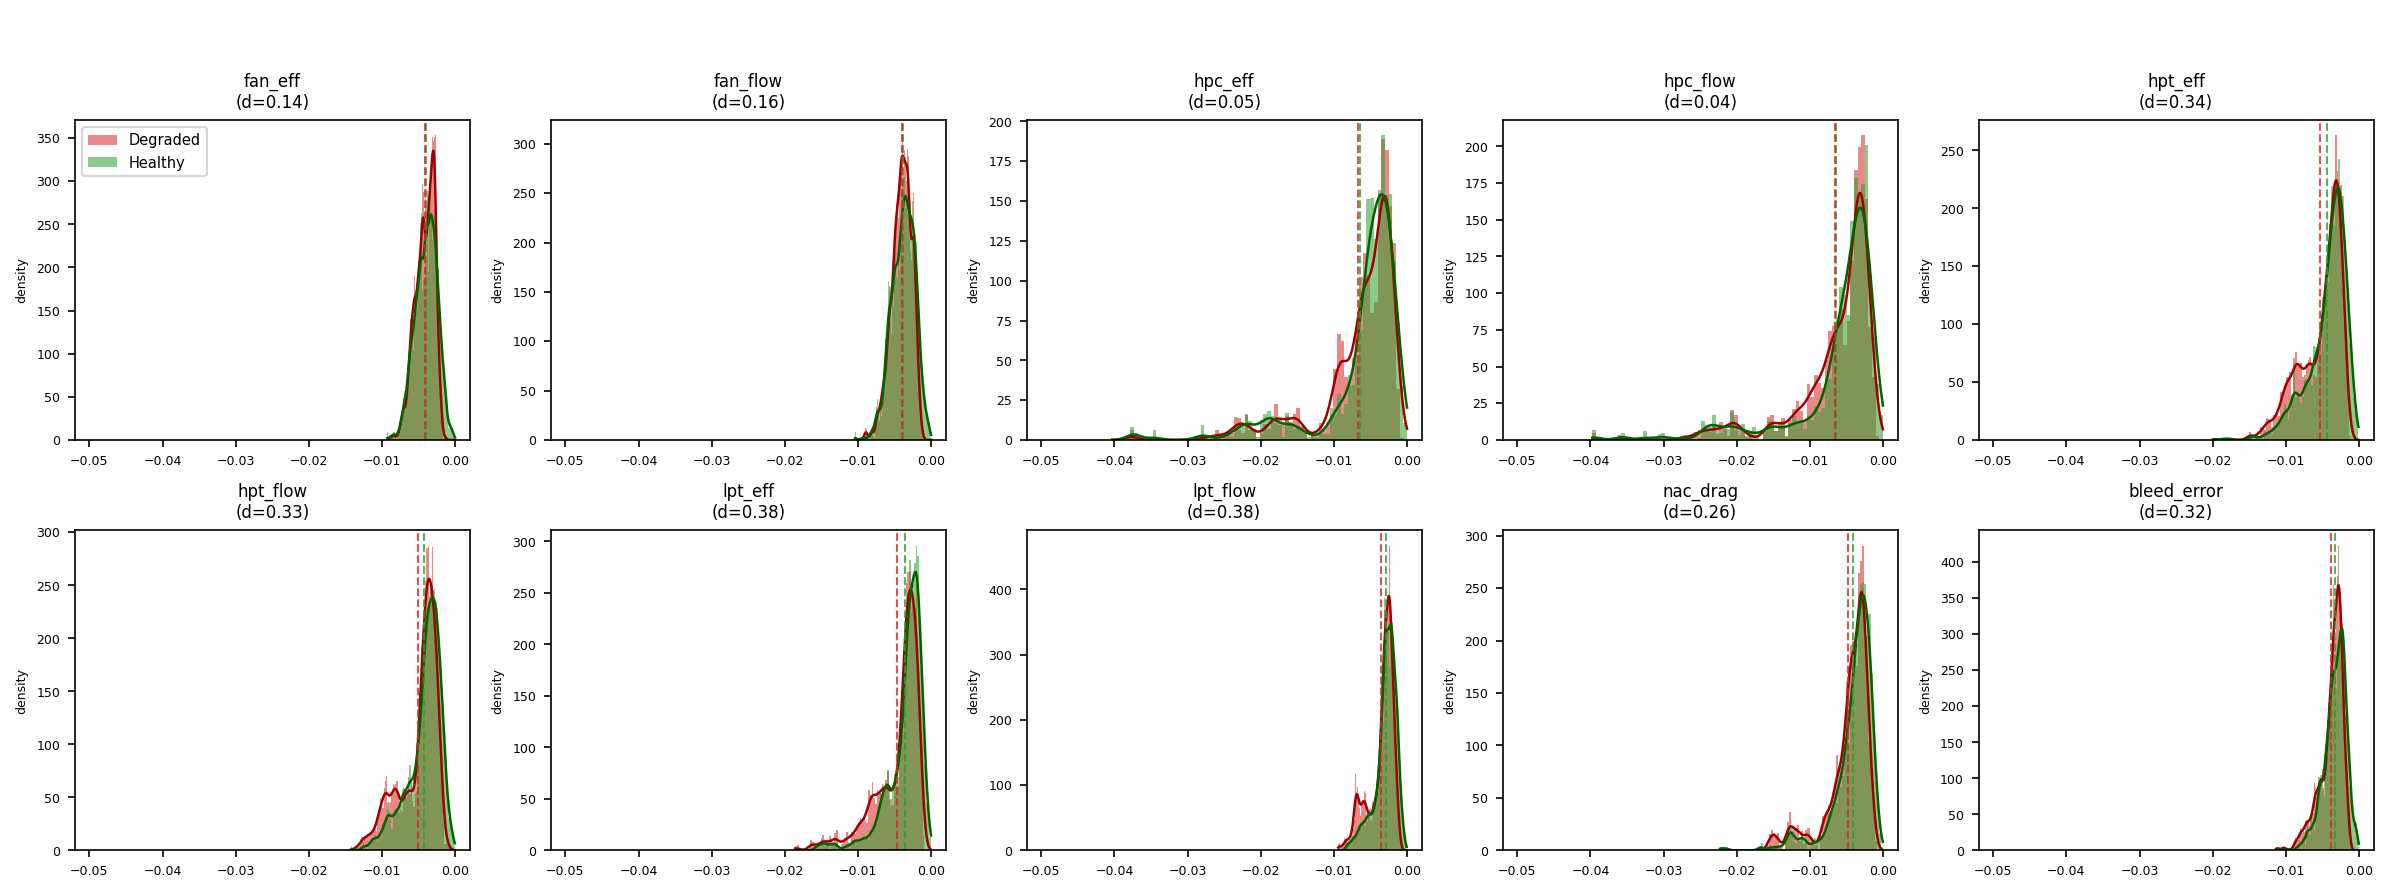
\includegraphics[width=\textwidth]{figures/eda_s3_state_healthy_degraded.png}
        \caption{Train set underlying state distribution between healthy and degraded.}
        \label{fig:healthy_degraded_train}
    \end{subfigure}
    
    \vspace{0.5em}
    
    \begin{subfigure}{\linewidth}
        \centering
        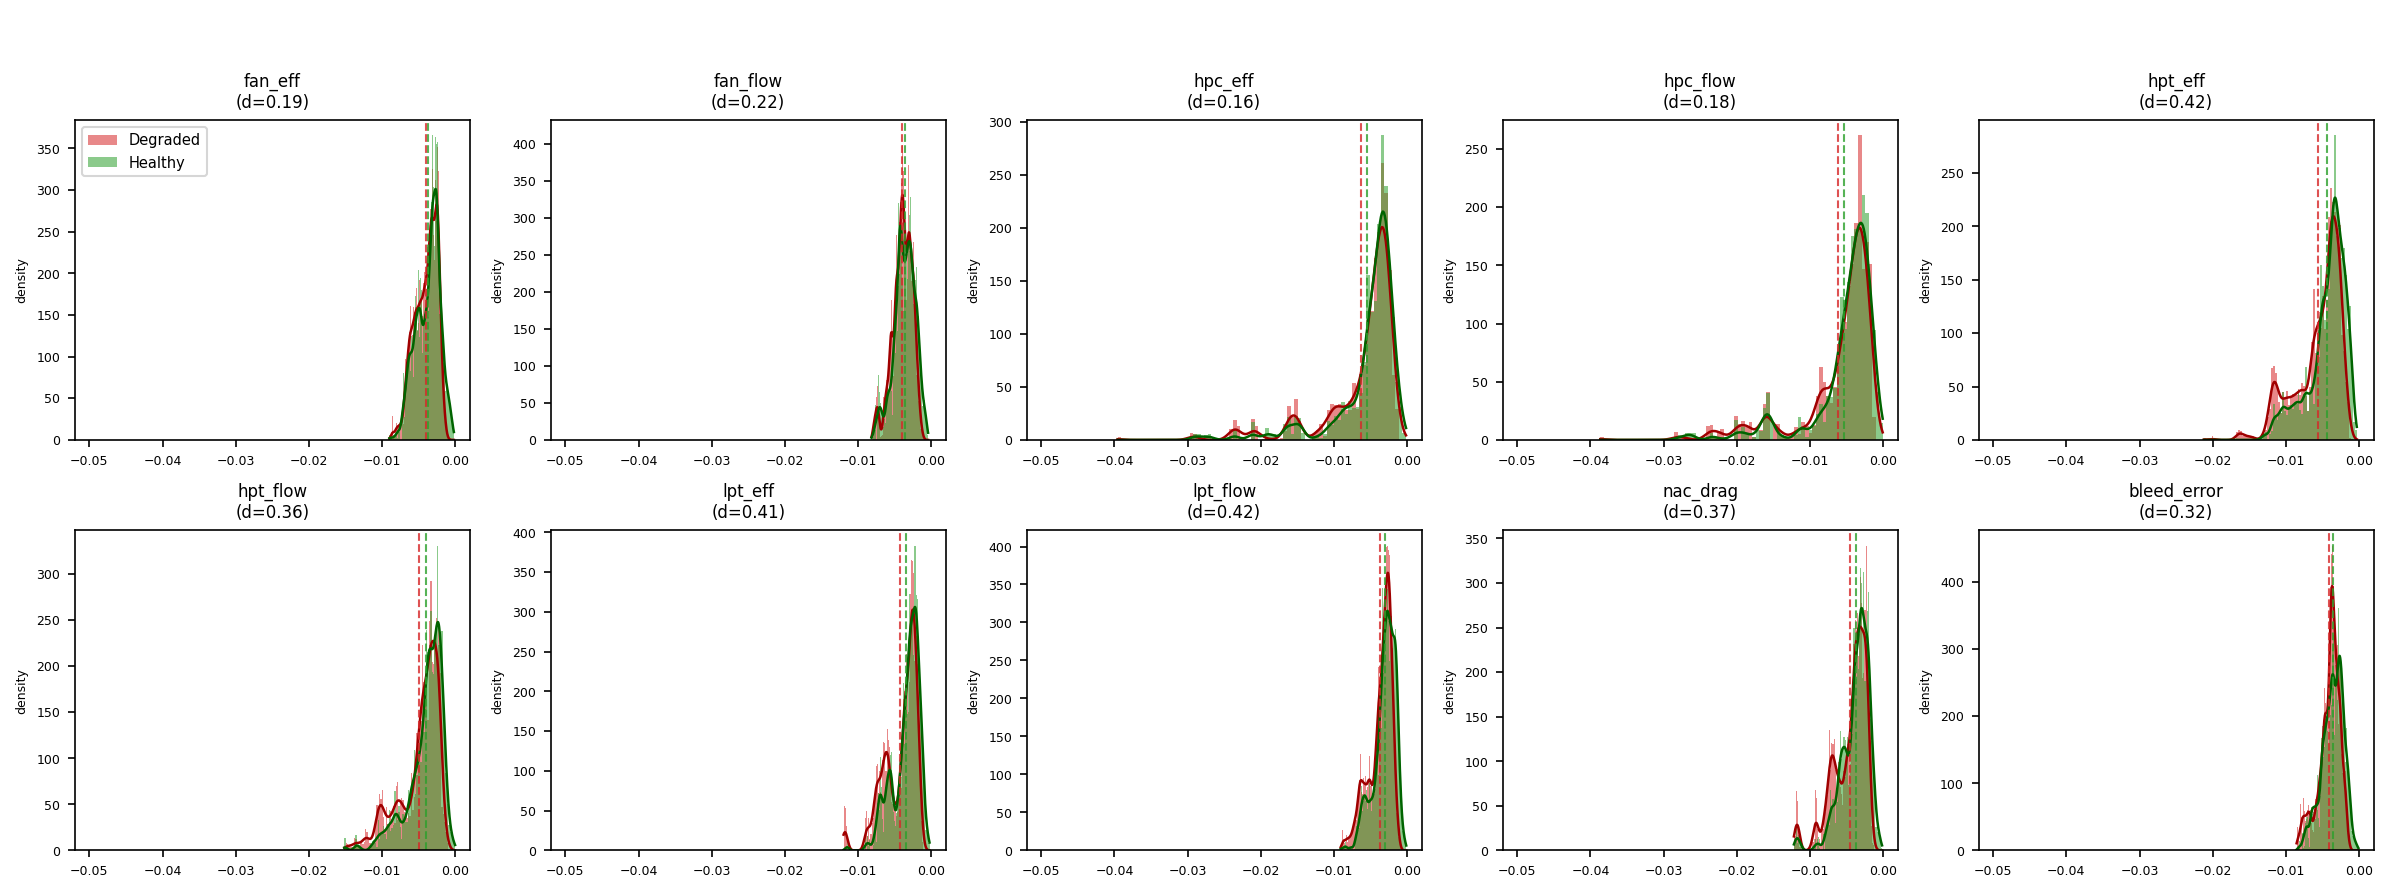
\includegraphics[width=\textwidth]{figures/eda_s3_state_healthy_degraded_test.png}
        \caption{Test set in‑distribution with train, between healthy and degraded.}
        \label{fig:healthy_degraded_test}
    \end{subfigure}
    
    \vspace{0.5em}
    
    \begin{subfigure}{\linewidth}
        \centering
        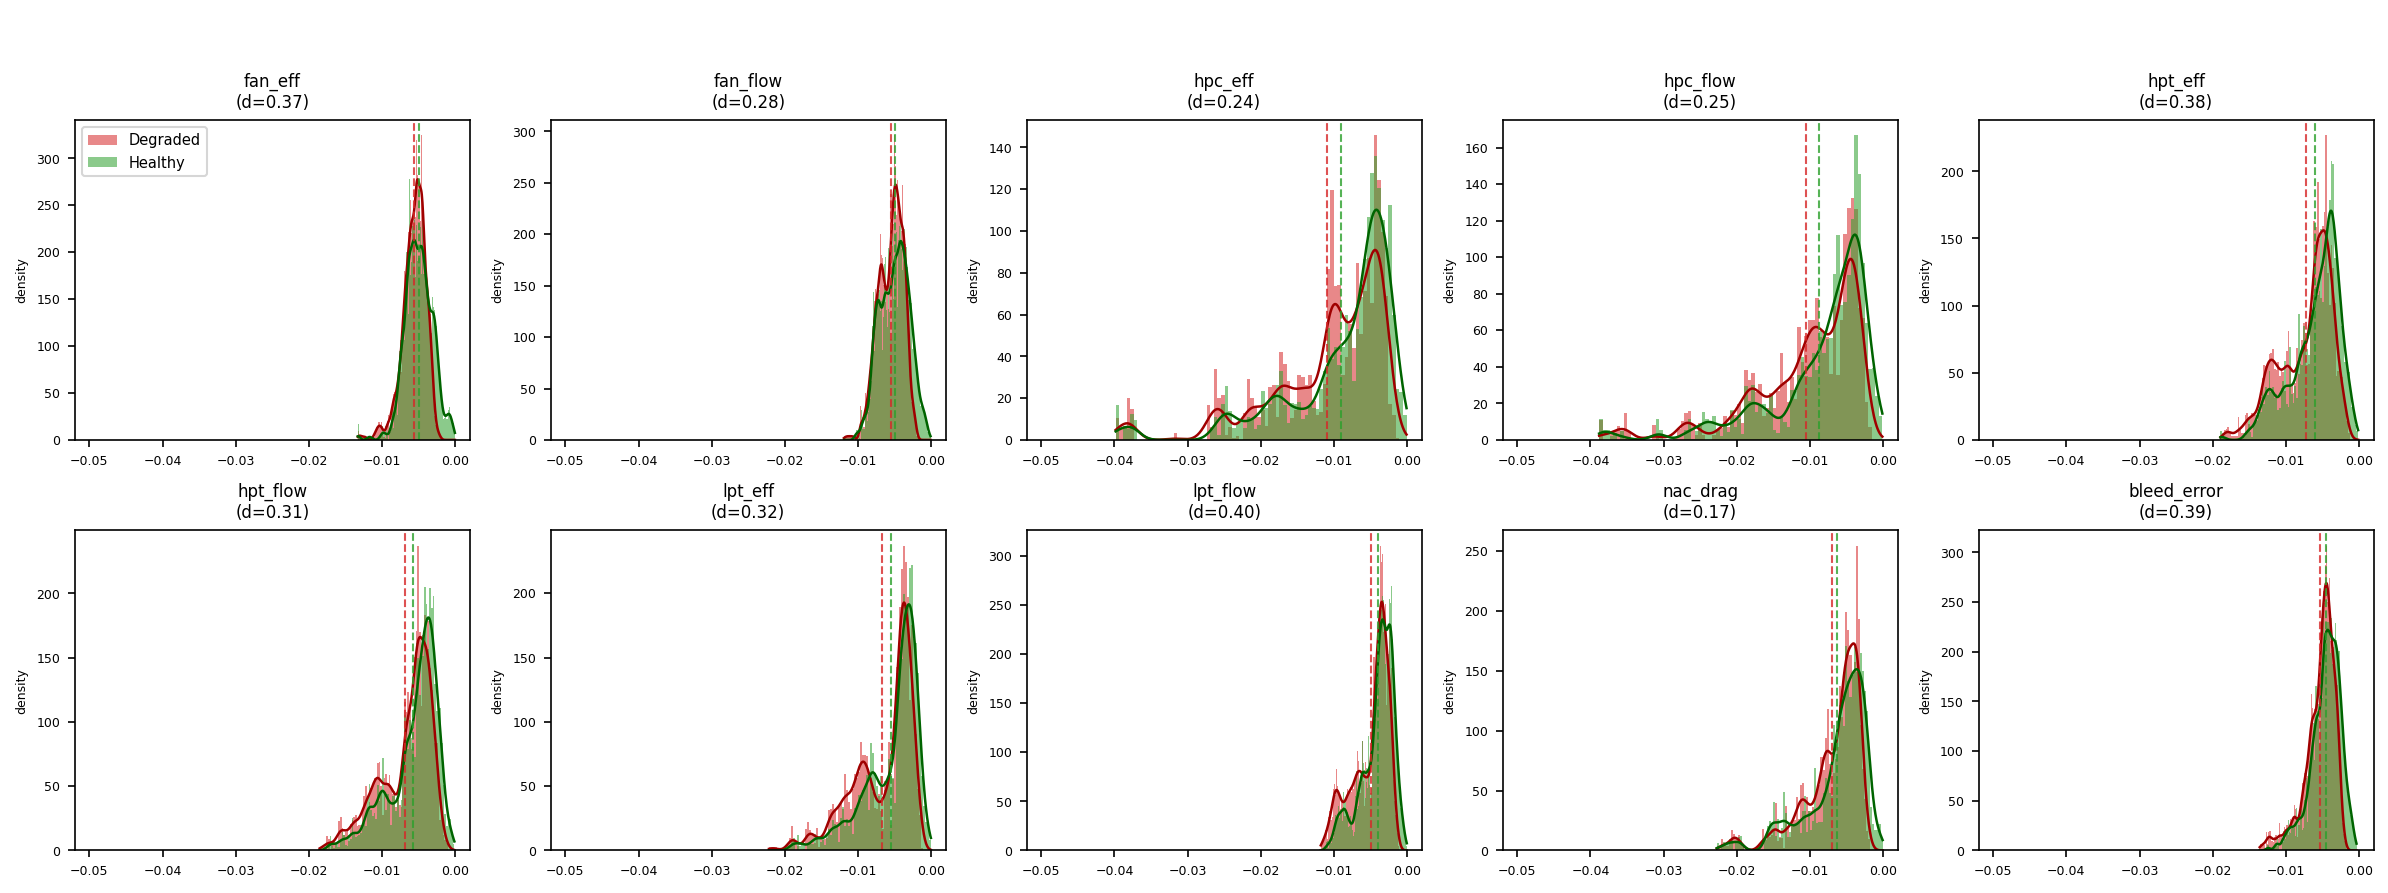
\includegraphics[width=\textwidth]{figures/eda_s3_state_healthy_degraded_test_hard.png}
        \caption{Test‑hard set out‑of‑distribution}
        \label{fig:healthy_degraded_test_hard}
    \end{subfigure}
    
    \caption{Distribution for Scenario 3 of the ten health‑state components under healthy (blue) and degraded (orange) regimes. Train and test share the same distribution; test‑hard introduces stronger degradation, varied drift rates, and modified maintenance to assess generalization beyond the training manifold.}
    \label{fig:healthy_degraded_all}
\end{figure}




% =============================================================================
%  TurboSens4 Dataset, LaTeX subsection (appendix version)
%  Compile inside a document that loads: amsmath, booktabs, multirow,
%  xcolor, hyperref (optional). Figures are referenced by label only;
%  include them wherever suitable in your document.
% =============================================================================

\subsection{TurboSens4: Regional Operating Environments and Contamination Dynamics}
\label{sec:dataset_scenario4}

TurboSens4 extends the Scenario~3 dataset along three physical axes that
are absent from existing turbofan benchmarks: the operating environment
in which an engine spends its service life, the separation between true
mechanical wear and reversible contamination of the gas path, and the
cross-module aerodynamic coupling that causes a locally damaged component
to make its neighbours appear healthier than they are. The scenario retains
the core ingredients of Scenario~3 (heterogeneous degradation archetypes,
life-limiting-part regulatory constraints, an imperfect expert maintenance
policy, a library of stochastic events, multi-context sensor observations
and a fully exposed hidden state) and layers on top of them a regional
operating model, a two-channel hidden state, a seasonal weather process
with realistic shop-visit downtimes, and an additional maintenance action
capturing periodic engine water washing.

The dataset is organised around six region archetypes, each representing
a distinct operating environment characterised by its dominant atmospheric
stressor (sand, salt, humidity, pollution, thermal swing). A region
archetype simultaneously biases the prior over degradation archetypes,
scales the mechanical drift rates of the most exposed sub-systems,
governs the contamination accumulation rate, restricts the library of
admissible stochastic events, and modulates the seasonal weather process
and the flight cadence. Between 80 and 400 episodes are generated per
region archetype, for a target total of approximately 1{,}500 episodes
with a mean length of 14{,}000 timesteps and a hard ceiling of 20{,}000
timesteps.

% -----------------------------------------------------------------------------
\subsubsection{Two-Channel Hidden State}
\label{sec:scen4_state}

\paragraph{Mechanical and contamination channels.}
The Scenario~3 hidden health state $\mathbf{s}_t \in \mathbb{R}^{10}$
is preserved and interpreted strictly as the \emph{mechanical} deviation
of efficiency and corrected flow from nominal for the five sub-systems
(Booster, Fan, HPC, HPT, LPT). Its evolution is driven solely by slow
stochastic wear (archetype-specific drift, burn-in transient, and
speed-regime noise); it is irreversible except through partial
restoration at shop visits. To capture the fast, reversible fouling
of the gas path we introduce a second hidden channel
$\mathbf{c}_t \in [0,1]^5$ encoding a normalised contamination level
per sub-system. Contamination accumulates each flight at a rate
conditioned on region, flight phase and active stochastic event set,
and resets to zero after any engine-wash action. Crucially, $\mathbf{c}_t$
does \emph{not} enter the mechanical state update: $\mathbf{s}_t$ and
$\mathbf{c}_t$ evolve on independent dynamics, representing two
physically distinct phenomena (material wear vs. surface deposition).

\paragraph{Observation model: the phantom state.}
The thermodynamic simulator produces sensor readings from an engine
state vector, so every hidden effect that modifies the gas-path flow
must enter the simulator through that vector. We therefore define a
\emph{phantom state} $\tilde{\mathbf{s}}_t \in \mathbb{R}^{10}$
that aggregates, on top of $\mathbf{s}_t$, the two observable-but-hidden
effects that the simulator cannot model intrinsically:
\begin{enumerate}
  \item \emph{Phantom flow coupling}: a breach or severe local wear
    redirects airflow through neighbouring modules, producing
    corrected-flow readings that are anomalously high for the
    healthy-looking neighbour while the true cause lies elsewhere.
  \item \emph{Contamination coupling}: surface fouling perturbs module
    efficiency and apparent flow even when the underlying mechanical
    state is pristine.
\end{enumerate}
Both effects are implemented as additive, non-negative couplings
clipped to the validated thermodynamic operating range:
\begin{equation}
  \tilde{s}^k_t \;=\; \mathrm{clip}\!\Bigl(
     s^k_t
     \;+\; \sum_{j=1}^{10} M_{kj}\,\max\!\bigl(0,\; -s^j_t\bigr)
     \;+\; \sum_{m=1}^{5} C_{km}\, c^m_t,
  \;\; \underline{b}_k,\; \overline{b}_k \Bigr),
  \quad k = 1,\ldots,10,
  \label{eq:phantom}
\end{equation}
where $M \in \mathbb{R}^{10 \times 10}$ is the sparse phantom
flow-coupling matrix of Scenario~3 (strictly positive entries only on
flow dimensions immediately downstream of each degrading efficiency
component), and $C \in \mathbb{R}^{10 \times 5}$ is a new sparse,
non-negative contamination-to-phantom matrix whose entry $C_{km}$ is
non-zero only when fouling of module $m$ physically perturbs state
dimension $k$ (for example, HPC fouling degrades HPC efficiency
and biases HPC flow upward). The mechanical-state bounds
$[\underline{b}_k, \overline{b}_k]$ are those used by the underlying
simulator: strictly non-positive on efficiency channels, and admitting
positive flow deviations up to $+0.03$ for Fan, Booster and HPC flow
and $+0.05$ for HPT and LPT flow. Coupling weights in $M$ and $C$ are
calibrated empirically to keep $\tilde{\mathbf{s}}_t$ within validated
thermodynamic ranges under all archetype and region combinations and
are exposed as named constants to support ablation studies; the
matrices are fixed across the dataset while $\mathbf{s}_t$ and
$\mathbf{c}_t$ vary per episode and timestep.

\paragraph{Final observation map.}
The simulator is queried on $\tilde{\mathbf{s}}_t$ rather than
$\mathbf{s}_t$, so contamination and phantom coupling both reach the
sensors through the same, physically grounded pathway, the state
vector that the thermodynamic model actually consumes:
\begin{equation}
  \mathbf{o}_t \;=\; g\!\bigl(\tilde{\mathbf{s}}_t, \omega_t\bigr)
  \;+\; \varepsilon_t,
  \label{eq:obs}
\end{equation}
where $g$ is the OpenDeckSMR thermodynamic model, $\omega_t$ collects
the ambient and command conditions of the flight context, and
$\varepsilon_t$ is residual sensor noise. Because $\mathbf{c}_t$ enters
the observation exclusively through $\tilde{\mathbf{s}}_t$ and is
reset by the engine-wash action while $\mathbf{s}_t$ is not, a wash
produces the characteristic sawtooth pattern in the sensor stream
while the underlying mechanical trajectory $\mathbf{s}_t$ is unaffected.
Both $\mathbf{c}_t$ and the phantom contribution $\tilde{\mathbf{s}}_t - \mathbf{s}_t$ are exposed in the  dataset metadata as per-step ground-truth labels, enabling supervised  evaluation of disentangling methods.

% -----------------------------------------------------------------------------
\subsubsection{Region Archetypes}
\label{sec:scen4_regions}

Each episode is assigned one of six region archetypes at generation
time (Table~\ref{tab:regions}). The names are deliberately
environmental rather than geographic. A region archetype determines four generation-time
parameters: (i) a prior over the four Scenario~3 degradation
archetypes, (ii) a per-subsystem mechanical drift scaling factor,
(iii) a baseline contamination accumulation rate, and (iv) a mean
flight cadence controlling how many simulated flights map to one
calendar day.

\begin{table}[h]
\centering
\caption{Region archetypes in TurboSens4. Severity is a qualitative
summary of combined mechanical and contamination load.}
\label{tab:regions}
\small
\begin{tabular}{llll}
\toprule
ID & Name & Dominant stressor & Severity \\
\midrule
R1 & Continental & None (baseline)               & Benign          \\
R2 & Littoral    & Salt spray, humidity          & Moderate        \\
R3 & Arid        & Sand, dust, thermal swing     & Harsh           \\
R4 & Equatorial  & Heat, humidity, bio-fouling   & Moderate        \\
R5 & Highland    & Cold ambient, thin air        & Benign-Moderate \\
R6 & Industrial  & Chemical pollution, soot      & Moderate-Harsh  \\
\bottomrule
\end{tabular}
\end{table}

\paragraph{Region-conditional archetype prior.}
The four Scenario~3 degradation archetypes (A compressor-driven,
B fan/booster-driven, C turbine-driven, D balanced) are retained
unchanged. Their prior probability is now conditioned on the region
(Table~\ref{tab:region_archetype_prior}), so that for instance Arid
over-represents A (sand erosion of the HPC) and Littoral over-represents
B (salt corrosion of the fan and booster).

\begin{table}[h]
\centering
\caption{Conditional prior $\mathbb{P}(\text{archetype}\mid\text{region})$
used at episode generation.}
\label{tab:region_archetype_prior}
\small
\begin{tabular}{lcccc}
\toprule
Region & A & B & C & D \\
\midrule
Continental & 0.30 & 0.20 & 0.25 & 0.25 \\
Littoral    & 0.20 & 0.40 & 0.20 & 0.20 \\
Arid        & 0.45 & 0.30 & 0.15 & 0.10 \\
Equatorial  & 0.30 & 0.30 & 0.20 & 0.20 \\
Highland    & 0.20 & 0.15 & 0.35 & 0.30 \\
Industrial  & 0.35 & 0.25 & 0.20 & 0.20 \\
\bottomrule
\end{tabular}
\end{table}

\paragraph{Per-subsystem mechanical scaling.}
Independently of the archetype, the region applies a multiplicative
scaling $\rho^{(r)}_k > 0$ to the drift rate $\alpha_k$ of
equation~\eqref{eq:deg_increment}, modelling the physical acceleration
of wear by the regional stressor (Table~\ref{tab:region_scaling}).
Littoral scales fan and booster drift, Arid scales HPC drift,
Highland shifts stress toward the thermal section.

\begin{table}[h]
\centering
\caption{Region-induced mechanical drift multipliers on $\alpha_k$ and
baseline contamination accumulation multiplier.}
\label{tab:region_scaling}
\small
\begin{tabular}{lcccc}
\toprule
Region & HPC & Fan / Booster & HPT / LPT & Contamination rate \\
\midrule
Continental & 1.0 & 1.0 & 1.0 & $1.0\times$ \\
Littoral    & 1.0 & 1.5 & 1.1 & $1.4\times$ \\
Arid        & 1.6 & 1.3 & 1.0 & $1.8\times$ \\
Equatorial  & 1.1 & 1.2 & 1.0 & $1.5\times$ \\
Highland    & 0.9 & 0.9 & 1.2 & $0.7\times$ \\
Industrial  & 1.2 & 1.2 & 1.1 & $1.6\times$ \\
\bottomrule
\end{tabular}
\end{table}

% -----------------------------------------------------------------------------
\subsubsection{Degradation and Contamination Dynamics}
\label{sec:scen4_degradation}

\paragraph{Extended mechanical increment.}
The Scenario~3 degradation increment~\eqref{eq:deg_increment} is
extended with two region-conditional terms: the region scaling
$\rho^{(r)}_k$ and a slow corrosion term driven by the accumulated
contamination,

\begin{equation}
  \Delta s^k_t \;=\; -\beta_k e^{-t_k/\tau_k}
                  \;-\; \rho^{(r)}_k\,\alpha^{(m)}_k
                  \;-\; \lambda_k\, c^{\pi(k)}_t
                  \;+\; \varepsilon_t,
  \label{eq:scen4_deg_increment}
\end{equation}

where $\pi(k) \in \{1,\ldots,5\}$ maps a state component to its
parent sub-system and $\lambda_k$ is a small corrosion coefficient
set so that a sub-system held at $c = 1$ for an entire episode would
contribute an additional drift of the same order as 15 to 20 percent
of the base archetype drift. Salt and sand therefore accelerate
mechanical wear only to the extent that cleaning is deferred.

\paragraph{Contamination increment.}
Contamination accumulates between maintenance visits at a rate
modulated by the region archetype and the flight phase of each of the
sixteen snapshot contexts seen within a step:

\begin{equation}
  \Delta c^\ell_t \;=\; \eta^{(r)}_\ell\, \sum_{i=1}^{16} w_{\phi_i}
                    \;-\; \delta\, c^\ell_t,
\end{equation}

where $\eta^{(r)}_\ell$ is the region-conditional deposition rate
(listed last column of Table~\ref{tab:region_scaling} after
normalisation by sub-system exposure), $w_{\phi_i}$ weights the
contribution of each snapshot context by its flight phase (takeoff and
climb deposit more than cruise), and $\delta$ is a small self-cleaning
term accounting for aerodynamic blow-off. Contamination is clipped to
$[0, 1]$ per sub-system.

Events (Section~\ref{sec:scen4_events}) can additionally apply a large
step increment to $\mathbf{c}_t$ (an \texttt{ingestion\_trans} or
\texttt{ingestion\_regional} event deposits a bulk of particulate onto
the HPC in a single step) or, for severe events such as
\texttt{ingestion\_perm}, a joint step change to both $\mathbf{s}_t$
and $\mathbf{c}_t$ that is visible in the snapshot at the event step.
The mapping between these labels and the physical phenomena they model
is given in Table~\ref{tab:event_nomenclature}.

\paragraph{Phantom-coupling interpretation.}
Because the phantom map~\eqref{eq:phantom} depends on the true state
$\mathbf{s}_t$, an episode in which a single efficiency dimension
degrades aggressively will exhibit a non-physical improvement in the
downstream flow dimension of a neighbouring module, followed by a
discontinuous return to nominal after maintenance restores the
efficiency. This provides a genuine counter-example to monotonic
degradation heuristics and serves as a latent-structure probe for
representation learning: a world model that has learned the true
mechanical state should detect the upstream efficiency loss as the
cause of the downstream flow excursion, whereas a purely local model
will mis-attribute the event.

% -----------------------------------------------------------------------------
\subsubsection{Maintenance Policy and Extended Action Set}
\label{sec:scen4_maintenance}

\paragraph{Engine water wash.}
A seventh maintenance action, \texttt{engine\_wash}, is added to the
original six Scenario~3 actions (Table~\ref{tab:scen4_actions}). A wash resets
the contamination vector $\mathbf{c}_t$ to zero (up to a small residual
noise), does not restore mechanical state, has a low cost (30 reward
units) and incurs only a short downtime (no multi-month calendar jump).
Wash timings are not triggered by health; they follow a semi-periodic
schedule per episode, with the mean wash interval drawn from
$[50, 150]$ steps for benign regions and $[30, 90]$ steps for harsh
regions, jittered by a per-wash noise term. This models the scheduled
maintenance practice of most commercial operators and produces the
sawtooth pattern in the observed sensor stream that our dataset is
designed to expose.

\begin{table}[h]
\centering
\caption{TurboSens4 maintenance actions. Actions 0 through 5 are
inherited from Scenario~3; action 6 is the new engine wash.}
\label{tab:scen4_actions}
\small
\begin{tabular}{llcp{4.7cm}}
\toprule
ID & Name & Cost & Target \\
\midrule
0 & \texttt{do\_nothing}       & 0   & None \\
1 & \texttt{fan\_overhaul}     & 150 & Fan Eff, Fan Wc \\
2 & \texttt{hpc\_overhaul}     & 200 & Booster Eff/Wc, HPC Eff/Wc \\
3 & \texttt{turbine\_overhaul} & 200 & HPT Eff/Wc, LPT Eff/Wc \\
4 & \texttt{full\_overhaul}    & 350 & All ten mechanical components \\
5 & \texttt{targeted\_patch}   &  80 & Most-degraded component (oracle) \\
6 & \texttt{engine\_wash}      &  30 & Reset $\mathbf{c}_t$ (contamination only) \\
\bottomrule
\end{tabular}
\end{table}

\paragraph{Shop-visit downtime and calendar jumps.}
Unlike Scenario~3, TurboSens4 represents the wall-clock cost of a
shop visit in the weather process rather than abstracting it away.
Each non-wash maintenance visit advances the episode calendar clock
by a duration drawn from a severity-dependent range: light targeted
patches add 0.5 to 1 month, mid-weight module overhauls add 2 to 3
months, and heavy or extreme-degradation overhauls add 5 months.
The seasonal weather state (Section~\ref{sec:scen4_weather}) jumps
forward accordingly at the next step, producing abrupt ambient
conditions transitions at the return from a shop visit that are a
distinctive feature of fleet operations. Contamination is reset to
zero at every maintenance visit, whether or not a wash action is
formally issued.

\paragraph{Seasonal modulation of proactive scheduling.}
Commercial operators defer non-critical maintenance during high-demand
summer flying seasons. This is captured by scaling the Scenario~3
proactive planning window $W_\mathrm{plan} \in [1500, 2500]$ by a
seasonal factor $\kappa_\mathrm{season}(t) \in [0.6, 1.3]$ that peaks
in local summer and is lowest in local winter. Life-limiting-part
ceilings and emergency thresholds are not subject to this seasonal
modulation: airworthiness-mandated replacement remains inflexible.

\paragraph{LLP and base policy structure.}
Life-limiting-part cycle limits are identical across all regions and
archetypes, reflecting their regulatory origin rather than any physical
susceptibility. Health-correlated scheduling, min-built bundling,
findings and imperfect restoration behave exactly as in Scenario~3,
operating on the mechanical state $\mathbf{s}_t$ and ignoring the
contamination channel $\mathbf{c}_t$. The wash action is handled as a
separate track that never interacts with the LLP counter and never
causes min-built bundling.

% -----------------------------------------------------------------------------
\subsubsection{Stochastic Event Library}
\label{sec:scen4_events}

The Scenario~3 event library is retained and extended with region
based gates on admissible events (see
Table~\ref{tab:event_nomenclature} for the mapping between labels and
their physical interpretation). \texttt{icing} is excluded in Arid and
Equatorial regions regardless of instantaneous weather, reflecting the
physical impossibility of in flight icing in hot environments.
\texttt{ingestion\_regional} is strongly over represented in Arid and
to a lesser extent Industrial regions. \texttt{corrosion\_regional},
introduced in Scenario~4 as a new event type, is gated to Littoral
and occasionally Equatorial. Events that jointly affect $\mathbf{s}_t$
and $\mathbf{c}_t$ (\texttt{ingestion\_perm} and
\texttt{ingestion\_regional}) apply their joint step change at the
event timestep, so that the snapshot observation at that step already
reflects the damaged engine.

The event rate per region is calibrated to keep the global stochastic
event rate below one percent of timesteps, preserving the sparsity
property that makes events challenging to detect. All event metadata
(type, timestep, affected components, magnitude) is exposed as
ground-truth labels for anomaly-detection and representation-probing
tasks.

% -----------------------------------------------------------------------------
\subsubsection{Flight Contexts}
\label{sec:scen4_contexts}

Each timestep is observed under $C = 16$ fixed flight contexts spanning
three physically supported phase types in OpenDeckSMR: cruise (CR),
max-climb (MCL) and take-off (MTO). The breakdown is eight nominal
cruise contexts spanning altitudes from 33{,}000 to 39{,}000 ft and
Mach numbers from 0.76 to 0.84, one low-power cruise context at
15{,}000 ft approximating an idle approach regime, four max-climb
contexts covering nominal, stepped, hot and cold variants, and three
take-off contexts covering nominal, hot-day and heavy-weight variants.
The low-power context is labelled as a low-thrust proxy rather than a
true descent phase because OpenDeckSMR does not validate thermodynamic
behaviour in the windmilling descent regime; its command value is
reduced to the lower bound of the CR envelope.

Each context remains internally consistent: take-off contexts combine
sea-level altitude with high ambient temperature and zero Mach, cruise
contexts combine high altitude with low ambient temperature and high
Mach, climb contexts span intermediate values. Cross-contaminating
context values (for example a cruise DTAMB applied at take-off altitude)
are explicitly forbidden by the sampler to keep every snapshot inside
the validated operating envelope of the physics simulator.

% -----------------------------------------------------------------------------
\subsubsection{Seasonal Weather Process}
\label{sec:scen4_weather}

TurboSens4 replaces the single-level Ornstein-Uhlenbeck weather process
of Scenario~3 with a three-level hierarchical generator that captures
seasonality, flight-to-flight variability and within-snapshot noise.

\paragraph{Seasonal baseline.}
A slow sinusoidal drift $\mu^{(r)}_\mathrm{season}(d_t)$ indexed by the
simulated calendar day $d_t$ models the region-specific annual cycle
of ambient temperature. Its amplitude is largest for Continental
(approximately $\pm 25$\,K peak-to-peak around the regional mean),
intermediate for Highland and Industrial, and smallest for Equatorial
(near-flat). The calendar day advances by $1 / \nu^{(r)}$ per timestep,
where $\nu^{(r)}$ is the region-conditional mean flight cadence:
Continental and Industrial at 4 to 5 flights per day, Littoral and
Equatorial at 2 to 3, Arid and Highland at 1 to 2, with per-region
jitter. Maintenance downtimes advance the calendar by the severity
dependent amount described in Section~\ref{sec:scen4_maintenance}.

\paragraph{Flight-level OU.}
Around the seasonal baseline, a faster OU process governs the weather
realised for one flight,

\begin{equation}
  d(\Delta T_\mathrm{flight})
    = \theta_\mathrm{f}\bigl(\mu^{(r)}_\mathrm{season}(d_t)
      - \Delta T_\mathrm{flight}\bigr)\, dt
      + \sigma_\mathrm{f}\, dW_t,
\end{equation}

with $\theta_\mathrm{f}$ chosen so the mean-reversion half-life covers
several flights and $\sigma_\mathrm{f}$ scaled to produce a realistic
day-to-day ambient dispersion. A fresh realisation is drawn at the
start of each simulated flight so that consecutive snapshots within a
flight share correlated weather, while consecutive flights can differ
substantially.

\paragraph{Within-snapshot jitter.}
A third small-amplitude Gaussian perturbation is finally added to
each of the sixteen snapshot contexts within a step, in addition to
the context-specific offsets documented in
Section~\ref{sec:scen4_contexts}. This captures turbulence and
small-scale atmospheric variability that differentiates the snapshots
even under an otherwise stable flight-level OU.

% -----------------------------------------------------------------------------
\subsubsection{Extreme-Degradation Episodes}
\label{sec:scen4_extreme}

A small fraction of episodes (between 1 and 5 percent)
are flagged as extreme-degradation episodes at generation time.
In these episodes the proactive policy's planning window and
emergency threshold are temporarily relaxed, allowing one or more
components to traverse a deep sag down to 92 to 95 percent of the
degradation bound before a heavy overhaul is dispatched. The overhaul
restores the affected components to between 88 and 95 percent of the
pristine bound, resets contamination, and advances the calendar clock
by five months. Extreme-degradation episodes are labelled and carry
metadata describing the sag window, the components involved, the
restoration quality and the post-visit calendar state. They are
deliberately rare so that reliable engines remain the statistical
norm, but are a vital stress test for prognostic methods that must
gracefully handle the upper tail of the degradation distribution.

% -----------------------------------------------------------------------------
\subsubsection{Ground-Truth Metadata}
\label{sec:scen4_metadata}

Every TurboSens4 episode carries a dense set of ground-truth labels
exposed alongside the sensor stream, making the dataset usable for
self-supervised pretraining, probing, anomaly detection and fine
grained diagnostic studies:

\begin{itemize}
\item Region archetype label $r \in \{\text{R1},\ldots,\text{R6}\}$
      and degradation archetype label $\in \{\text{A,B,C,D}\}$.
\item Mechanical state trajectory $\mathbf{s}_t \in \mathbb{R}^{10}$
      and contamination trajectory $\mathbf{c}_t \in \mathbb{R}^{5}$
      at every step.
\item Phantom-coupled state $\tilde{\mathbf{s}}_t$ and the coupling
      matrix $M$ used to generate it.
\item Action label $a_t \in \{0,\ldots,6\}$ including the new wash
      action, together with the Scenario~3 extended action metadata
      (component-service mask, visit-type flag, finding count).
\item Stochastic event mask and per-event parameters.
\item Simulated calendar day $d_t$, season label, and flag indicating
      whether the step follows a shop-visit calendar jump.
\item Flight cadence $\nu^{(r)}$ realised for the episode, wash-schedule
      timings, and an extreme-degradation boolean flag.
\end{itemize}

% -----------------------------------------------------------------------------
\subsubsection{Dataset Statistics}
\label{sec:scen4_stats}

Table~\ref{tab:scen4_summary} summarises the target properties of the
TurboSens4 release. The values are the current design targets;
observed statistics will be reported after the first full generation
run.

\begin{table}[h]
\centering
\caption{TurboSens4 target dataset statistics.}
\label{tab:scen4_summary}
\small
\begin{tabular}{lr}
\toprule
Property & Value \\
\midrule
Region archetypes                  & 6 \\
Episodes per region                & 80 to 400 \\
Total target episodes              & $\approx 1{,}500$ \\
Mean episode length                & 14{,}000 steps \\
Maximum episode length             & 20{,}000 steps \\
Number of flight contexts          & 16 \\
Maintenance actions                & 7 (including engine wash) \\
Mechanical state dimension         & 10 \\
Contamination state dimension      & 5 \\
Phantom coupling matrix $M$        & fixed, sparse non-negative \\
Extreme-degradation episode rate   & 1 to 5 percent \\
Stochastic event rate              & below 1 percent of timesteps \\
Sensor observation shape           & $(N, 7, 16)$ \\
On-disk size (HDF5, gzip)          & 8 to 12 GB (estimated) \\
\bottomrule
\end{tabular}
\end{table}








\section{Architecture and Implementation Details}
\label{app:architecture}

\subsection{Sensor Encoder}
\label{app:sensor_encoder}

Table~\ref{tab:sensor_encoder} summarises the sensor encoder hyperparameters
used in all reported experiments.
The Pre-LayerNorm variant (norm applied \emph{before} each sub-layer)
is used throughout for training stability~\citep{xiong2020layer}.
The embedding dimension $d{=}64$ is deliberately kept small to match
the world-model latent size and avoid introducing an unnecessary projection
bottleneck: the output of the sensor encoder is passed through a two-layer
MLP projector (hidden size 2048, BatchNorm) before entering the JEPA
predictor.

\begin{table}[h]
  \centering
  \caption{Sensor encoder configuration.}
  \label{tab:sensor_encoder}
  \begin{tabular}{ll}
    \toprule
    Hyperparameter & Value \\
    \midrule
    Input tokens ($n_\text{sensors}$) & 28 (4 contexts $\times$ 7 channels) \\
    Embedding dimension $d$ & 64 \\
    Attention heads & 4 \\
    Transformer layers $L$ & 2 \\
    Feed-forward multiplier & 4$\times$ \\
    Normalisation & Pre-LayerNorm \\
    Dropout & 0.1 \\
    Positional encoding & Learnable \\
    Pooling & Mean over tokens \\
    \bottomrule
  \end{tabular}
\end{table}

\subsection{Temporal Aggregator}
\label{app:temporal_agg}

For window size $w > 1$, a lightweight Temporal Aggregator
(Eq.~\eqref{eq:temporal_agg} in the main text) fuses $w$ consecutive
per-frame embeddings into a single trajectory-aware representation.
The aggregator is a one-layer transformer encoder (batch-first,
$d{=}64$, 4 heads) with learnable positional embeddings for positions
$0, \ldots, w_\text{max}-1$.
The output at the \emph{last} position (most recent frame) is used as the
aggregated embedding; this token attends over the full window and hence
receives information from the entire $w$-step trajectory.
The total number of parameters added by the aggregator is
$\mathcal{O}(d^2)$, negligible relative to the predictor.

The effective dataset loading changes with $w$: each training sample
contains $T_\text{raw} = H + n_\text{pred} + w - 1$ frames, from which
$T_\text{out} = H + n_\text{pred}$ output embeddings are produced via
a sliding-window scan.
Action embeddings are aligned by selecting the $w{-}1, \ldots, T_\text{raw}-1$
positions from the full action-embedding sequence.


\subsection{World Model Architecture}
\label{sec:architecture}

\paragraph{Observation representation.}
A single turbofan observation $\mathbf{o}_t \in \mathbb{R}^{n_s}$, with
$n_s = S \cdot C$, consists of $S{=}7$ sensor channels each measured under
$C$ flight-phase contexts, all reflecting the \emph{same} degradation state
at timestep~$t$.
For TurboSens3, $C{=}12$ contexts yield $n_s{=}84$.
Prior work encoded this vector as a grayscale image and applied a Vision
Transformer (ViT)~\citep{dosovitskiy2021image} after nearest-neighbour
upsampling, introducing significant inductive bias mismatch: patch-based
tokenisation is designed for spatially structured images, whereas turbofan
sensor readings are unordered scalar channels with no meaningful spatial
layout.
We therefore replace this pipeline with a \emph{sensor-native transformer}
that treats each of the $n_s$ scalar values as an independent token
(Section~\ref{sec:sensor_encoder}).

\paragraph{Sensor encoder.}
\label{sec:sensor_encoder}
Our encoder $\mathrm{Enc}_\theta : \mathbb{R}^{n_s} \to \mathbb{R}^d$ projects each
scalar $x_i$ to a $d$-dimensional token via a shared linear layer, adds a
learnable positional embedding, processes the resulting $n_s$-token sequence
through an $L$-layer Pre-LayerNorm Transformer~\citep{xiong2020layer}, and
mean-pools the output tokens:
\begin{equation}
  \mathbf{z}_t = \mathrm{LayerNorm}\!\left(
    \frac{1}{n_s}\sum_{i=1}^{n_s}
      \mathrm{TF}_\theta\!\left(
        \mathbf{W}_v\, x_{t,i} + \mathbf{p}_i
      \right)
  \right), \quad \mathbf{z}_t \in \mathbb{R}^d.
  \label{eq:sensor_encoder}
\end{equation}

\paragraph{Temporal depth.}
\label{sec:temporal_depth}
The encoder in Eq.~\eqref{eq:sensor_encoder} operates on a single snapshot and therefore cannot directly capture degradation rate or trend direction.
We introduce an encoder-level temporal window of size $w$: the encoder processes each of the $w$ consecutive frames $\mathbf{o}_{t-w+1}, \ldots, \mathbf{o}_t$ independently with shared weights, producing per-frame embeddings $\mathbf{z}_{t-w+1}, \ldots, \mathbf{z}_t$.
A lightweight Temporal Aggregator, a single-layer transformer that
takes the $w$-token sequence and returns the last-token output, then
compresses the window into one trajectory-aware embedding
$\mathbf{z}^\mathrm{agg}_t \in \mathbb{R}^d$:
\begin{equation}
  \mathbf{z}^\mathrm{agg}_t = \mathrm{TempAgg}\!\left(
    \mathbf{z}_{t-w+1}, \ldots, \mathbf{z}_t
  \right).
  \label{eq:temporal_agg}
\end{equation}
Setting $w{=}1$ recovers the snapshot baseline with no aggregation.
We study $w \in \{1, 5, 10\}$ as an ablation (Section~\ref{sec:ablation}).

\paragraph{JEPA world model.}
The world model follows the Joint-Embedding Predictive Architecture
(JEPA, LeWM)~\citep{Balestriero_LeCun_2025, Maes_Lidec_Scieur_LeCun_Balestriero_2026}.
Given a context window of $H$ consecutive embeddings
$\mathbf{z}^\mathrm{agg}_{t-H+1}, \ldots, \mathbf{z}^\mathrm{agg}_t$ and the
corresponding action embeddings, an autoregressive predictor
$g_\psi$ predicts the next embedding $\mathbf{z}^\mathrm{agg}_{t+1}$ in latent
space.
The full training objective combines a JEPA prediction loss with a
Signal Regularity (SIGReg) term~\citep{CITE} that encourages
the learned latent space to follow an isotropic Gaussian distribution,
preventing representational collapse:
\begin{equation}
  \mathcal{L} = \underbrace{
    \left\lVert g_\psi(\mathbf{z}^\mathrm{agg}_{t-H:t},\, \mathbf{a}_{t-H:t})
      - \mathbf{z}^\mathrm{agg}_{t+1} \right\rVert_2^2
  }_{\text{prediction loss}}
  \;\;+\;\;
  \lambda \cdot \mathcal{L}_{\mathrm{SIGReg}}.
  \label{eq:loss}
\end{equation}






\subsection{Predictor}
\label{app:predictor}

The autoregressive predictor $g_\psi$ is a causal transformer
(depth 4, 8 heads, MLP dimension 512, head dimension 32) that takes
the history of $H{=}3$ embeddings and their corresponding action embeddings
as input and outputs one predicted next-step embedding.
A second MLP projector (same architecture as the encoder projector) maps
the predictor output back to the shared $d$-dimensional latent space.

\subsection{Training Setup}
\label{app:training}

All models are trained for 100 epochs with AdamW ($\text{lr}=7{\times}10^{-5}$,
weight decay $10^{-3}$) under a LinearWarmup-CosineAnnealing schedule.
We use mixed-precision training (\texttt{fp16}) rather than \texttt{bfloat16}:
in early experiments the 3-decimal-digit dynamic range of \texttt{bf16}
produced silent overflows in the SIGReg operation, manifesting as a sudden
spike in validation loss at epochs 7--8.
Gradient clipping (global norm $0.3$) provides additional early-epoch
stability before the cosine schedule begins to decay the learning rate.
All runs use a single H100 GPU with batch size 128.

\begin{table}[h]
  \centering
  \caption{Training hyperparameters.}
  \label{tab:training}
  \begin{tabular}{ll}
    \toprule
    Hyperparameter & Value \\
    \midrule
    Optimiser & AdamW \\
    Learning rate & $7{\times}10^{-5}$ \\
    Weight decay & $10^{-3}$ \\
    LR schedule & LinearWarmup + CosineAnnealing \\
    Gradient clip (global norm) & 0.3 \\
    Batch size & 128 \\
    Epochs & 100 \\
    Precision & fp16-mixed \\
    SIGReg weight $\lambda$ & 0.15 \\
    SIGReg knots / projections & 17 / 1024 \\
    History $H$ & 1,3,10,50 \\
    \bottomrule
  \end{tabular}
\end{table}

\subsection{Downstream Evaluation Probes}
\label{app:probes}

\paragraph{Health Indicator (HI) probe.}
After every $k{=}5$ training epochs we freeze the encoder and train a
lightweight transformer regression head (2-layer, $d{=}64$, 4 heads) on
top of the frozen embeddings to predict the 10 turbofan Health Indicator
(HI) dimensions simultaneously.
The probe is trained with Adam ($\text{lr}{=}10^{-3}$) for up to 150 epochs
with early stopping (patience 20) on mean per-dimension RMSE.
We report per-component $R^2$, RMSE, and Pearson-$r$.

We evaluate two configurations to disentangle encoder-level from
probe-level temporal reasoning:
\begin{itemize}
  \item \textbf{seq\_len=1}: each probe input is a single frozen embedding
    (i.e.\ a snapshot).  Self-attention is trivial; the probe is functionally
    an MLP.  This directly measures what the \emph{encoder} has learned.
  \item \textbf{seq\_len=10}: each input is a window of 10 consecutive
    embeddings.  The probe transformer can attend over the trajectory,
    partially compensating for a snapshot encoder.  Comparing seq\_len=1
    \emph{vs.} seq\_len=10 reveals how much temporal context is already
    baked into the encoder embeddings.
\end{itemize}

\paragraph{Action-RUL probe.}
We additionally train a single-output regression probe to predict
$\tau_t = \min(\text{steps to next maintenance action}, \tau_\text{max})$,
with $\tau_\text{max}{=}300$.
Targets are log1p-transformed and StandardScaler-normalised before training.
Because $\sim$19\% of timesteps have no future maintenance event within the
horizon (censored, $\tau_t = \tau_\text{max}$), evaluation metrics (RMSE,
MAE, $R^2$, Pearson-$r$) are computed exclusively on the uncensored subset
($\tau_t < \tau_\text{max}$).
We report the fraction of uncensored test samples alongside the metrics.



\subsubsection{What each parameter actually controls}

\begin{table}[]
    \centering
    \begin{tabular}{|p{3cm}|p{3cm}|p{3cm}|p{3cm}|} \hline
        \textbf{Parameter} & \textbf{Affects Encoder?} & \textbf{Affects Predictor?} & \textbf{Affects Probe?} \\ \hline
        $w$ (observation window size) &
        \textbf{Yes}, the depth of temporal fusion inside $z_t$ &
        Indirectly, richer $z_t$ creates a different loss surface &
        Indirectly \\ \hline

        $H$ (history size) &
        \textbf{Yes}, how many past $z$'s the predictor sees &
        No &
        No \\ \hline

        $\text{seq\_len}$ &
        No &
        No &
        \textbf{Yes}, window fed to the probe head \\ \hline
    \end{tabular}
    \caption{What each temporal hyperparameter actually controls in the architecture.}
    \label{tab:temp_hyperparams}
\end{table}


\subsection{Additional Tasks that can be done}

\begin{enumerate}
    \item Conformal predicito
    \item New datasets
    \item Transfer Learning
    \item RL policy optimization
\end{enumerate}





\newpage
\input{checklist.tex}



\end{document}